\documentclass[twoside]{book}

% Packages required by doxygen
\usepackage{fixltx2e}
\usepackage{calc}
\usepackage{doxygen}
\usepackage[export]{adjustbox} % also loads graphicx
\usepackage{graphicx}
\usepackage[utf8]{inputenc}
\usepackage{makeidx}
\usepackage{multicol}
\usepackage{multirow}
\PassOptionsToPackage{warn}{textcomp}
\usepackage{textcomp}
\usepackage[nointegrals]{wasysym}
\usepackage[table]{xcolor}

% NLS support packages
\usepackage[french]{babel}

% Font selection
\usepackage[T1]{fontenc}
\usepackage[scaled=.90]{helvet}
\usepackage{courier}
\usepackage{amssymb}
\usepackage{sectsty}
\renewcommand{\familydefault}{\sfdefault}
\allsectionsfont{%
  \fontseries{bc}\selectfont%
  \color{darkgray}%
}
\renewcommand{\DoxyLabelFont}{%
  \fontseries{bc}\selectfont%
  \color{darkgray}%
}
\newcommand{\+}{\discretionary{\mbox{\scriptsize$\hookleftarrow$}}{}{}}

% Page & text layout
\usepackage{geometry}
\geometry{%
  a4paper,%
  top=2.5cm,%
  bottom=2.5cm,%
  left=2.5cm,%
  right=2.5cm%
}
\tolerance=750
\hfuzz=15pt
\hbadness=750
\setlength{\emergencystretch}{15pt}
\setlength{\parindent}{0cm}
\setlength{\parskip}{0.2cm}
\makeatletter
\renewcommand{\paragraph}{%
  \@startsection{paragraph}{4}{0ex}{-1.0ex}{1.0ex}{%
    \normalfont\normalsize\bfseries\SS@parafont%
  }%
}
\renewcommand{\subparagraph}{%
  \@startsection{subparagraph}{5}{0ex}{-1.0ex}{1.0ex}{%
    \normalfont\normalsize\bfseries\SS@subparafont%
  }%
}
\makeatother

% Headers & footers
\usepackage{fancyhdr}
\pagestyle{fancyplain}
\fancyhead[LE]{\fancyplain{}{\bfseries\thepage}}
\fancyhead[CE]{\fancyplain{}{}}
\fancyhead[RE]{\fancyplain{}{\bfseries\leftmark}}
\fancyhead[LO]{\fancyplain{}{\bfseries\rightmark}}
\fancyhead[CO]{\fancyplain{}{}}
\fancyhead[RO]{\fancyplain{}{\bfseries\thepage}}
\fancyfoot[LE]{\fancyplain{}{}}
\fancyfoot[CE]{\fancyplain{}{}}
\fancyfoot[RE]{\fancyplain{}{\bfseries\scriptsize Généré le Vendredi 11 Mars 2016 00\+:27\+:09 pour Fractale par Doxygen }}
\fancyfoot[LO]{\fancyplain{}{\bfseries\scriptsize Généré le Vendredi 11 Mars 2016 00\+:27\+:09 pour Fractale par Doxygen }}
\fancyfoot[CO]{\fancyplain{}{}}
\fancyfoot[RO]{\fancyplain{}{}}
\renewcommand{\footrulewidth}{0.4pt}
\renewcommand{\chaptermark}[1]{%
  \markboth{#1}{}%
}
\renewcommand{\sectionmark}[1]{%
  \markright{\thesection\ #1}%
}

% Indices & bibliography
\usepackage{natbib}
\usepackage[titles]{tocloft}
\setcounter{tocdepth}{3}
\setcounter{secnumdepth}{5}
\makeindex

% Hyperlinks (required, but should be loaded last)
\usepackage{ifpdf}
\ifpdf
  \usepackage[pdftex,pagebackref=true]{hyperref}
\else
  \usepackage[ps2pdf,pagebackref=true]{hyperref}
\fi
\hypersetup{%
  colorlinks=true,%
  linkcolor=blue,%
  citecolor=blue,%
  unicode%
}

% Custom commands
\newcommand{\clearemptydoublepage}{%
  \newpage{\pagestyle{empty}\cleardoublepage}%
}


%===== C O N T E N T S =====

\begin{document}

% Titlepage & ToC
\hypersetup{pageanchor=false,
             bookmarks=true,
             bookmarksnumbered=true,
             pdfencoding=unicode
            }
\pagenumbering{roman}
\begin{titlepage}
\vspace*{7cm}
\begin{center}%
{\Large Fractale }\\
\vspace*{1cm}
{\large Généré par Doxygen 1.8.9.1}\\
\vspace*{0.5cm}
{\small Vendredi 11 Mars 2016 00:27:09}\\
\end{center}
\end{titlepage}
\clearemptydoublepage
\tableofcontents
\clearemptydoublepage
\pagenumbering{arabic}
\hypersetup{pageanchor=true}

%--- Begin generated contents ---
\chapter{Index hiérarchique}
\section{Hiérarchie des classes}
Cette liste d\textquotesingle{}héritage est classée approximativement par ordre alphabétique \+:\begin{DoxyCompactList}
\item \contentsline{section}{Application}{\pageref{class_application}}{}
\begin{DoxyCompactList}
\item \contentsline{section}{Homothetie}{\pageref{class_homothetie}}{}
\item \contentsline{section}{Rotation}{\pageref{class_rotation}}{}
\item \contentsline{section}{Similitude\+Directe}{\pageref{class_similitude_directe}}{}
\item \contentsline{section}{Similitude\+Indirecte}{\pageref{class_similitude_indirecte}}{}
\end{DoxyCompactList}
\item \contentsline{section}{Forme}{\pageref{class_forme}}{}
\item \contentsline{section}{Fractale}{\pageref{class_fractale}}{}
\item \contentsline{section}{Q\+Main\+Window}{\pageref{class_q_main_window}}{}
\begin{DoxyCompactList}
\item \contentsline{section}{Window}{\pageref{class_window}}{}
\end{DoxyCompactList}
\end{DoxyCompactList}

\chapter{Index des classes}
\section{Liste des classes}
Liste des classes, structures, unions et interfaces avec une brève description \+:\begin{DoxyCompactList}
\item\contentsline{section}{\hyperlink{class_application}{Application} }{\pageref{class_application}}{}
\item\contentsline{section}{\hyperlink{class_forme}{Forme} }{\pageref{class_forme}}{}
\item\contentsline{section}{\hyperlink{class_fractale}{Fractale} }{\pageref{class_fractale}}{}
\item\contentsline{section}{\hyperlink{class_homothetie}{Homothetie} }{\pageref{class_homothetie}}{}
\item\contentsline{section}{\hyperlink{class_q_main_window}{Q\+Main\+Window} }{\pageref{class_q_main_window}}{}
\item\contentsline{section}{\hyperlink{class_rotation}{Rotation} }{\pageref{class_rotation}}{}
\item\contentsline{section}{\hyperlink{class_similitude_directe}{Similitude\+Directe} }{\pageref{class_similitude_directe}}{}
\item\contentsline{section}{\hyperlink{class_similitude_indirecte}{Similitude\+Indirecte} }{\pageref{class_similitude_indirecte}}{}
\item\contentsline{section}{\hyperlink{class_window}{Window} }{\pageref{class_window}}{}
\end{DoxyCompactList}

\chapter{Documentation des classes}
\hypertarget{class_application}{}\section{Référence de la classe Application}
\label{class_application}\index{Application@{Application}}


{\ttfamily \#include \char`\"{}application.\+h\char`\"{}}



Graphe d\textquotesingle{}héritage de Application\+:\nopagebreak
\begin{figure}[H]
\begin{center}
\leavevmode
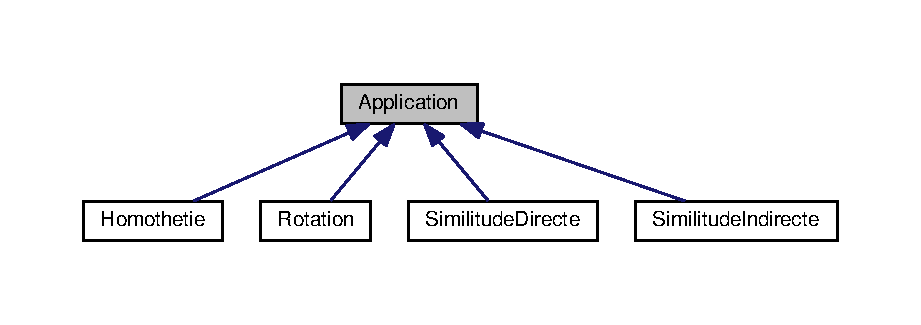
\includegraphics[width=350pt]{class_application__inherit__graph}
\end{center}
\end{figure}


Graphe de collaboration de Application\+:\nopagebreak
\begin{figure}[H]
\begin{center}
\leavevmode
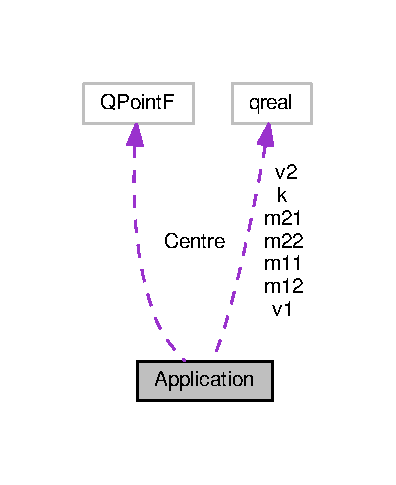
\includegraphics[width=190pt]{class_application__coll__graph}
\end{center}
\end{figure}
\subsection*{Fonctions membres publiques}
\begin{DoxyCompactItemize}
\item 
\hyperlink{class_application_afa8cc05ce6b6092be5ecdfdae44e05f8}{Application} ()
\begin{DoxyCompactList}\small\item\em \hyperlink{class_application_afa8cc05ce6b6092be5ecdfdae44e05f8}{Application\+::\+Application} Constructeur par default de \hyperlink{class_application}{Application}. \end{DoxyCompactList}\item 
void \hyperlink{class_application_a6497226f03c582468906c2752fb3e604}{setm11} (qreal m)
\begin{DoxyCompactList}\small\item\em \hyperlink{class_application_a6497226f03c582468906c2752fb3e604}{Application\+::setm11}. \end{DoxyCompactList}\item 
void \hyperlink{class_application_abf90c1d5903aa1ae2d4bfb05922f5742}{setm12} (qreal m)
\begin{DoxyCompactList}\small\item\em \hyperlink{class_application_abf90c1d5903aa1ae2d4bfb05922f5742}{Application\+::setm12}. \end{DoxyCompactList}\item 
void \hyperlink{class_application_a9aed2c898106e2f7bb32c115860415d1}{setm21} (qreal m)
\begin{DoxyCompactList}\small\item\em \hyperlink{class_application_a9aed2c898106e2f7bb32c115860415d1}{Application\+::setm21}. \end{DoxyCompactList}\item 
void \hyperlink{class_application_a32c06028e2ad3396d49fec90db0e51ac}{setm22} (qreal m)
\begin{DoxyCompactList}\small\item\em \hyperlink{class_application_a32c06028e2ad3396d49fec90db0e51ac}{Application\+::setm22}. \end{DoxyCompactList}\item 
void \hyperlink{class_application_a71f187ec6cbb5be46a9c56c8997b7295}{setv1} (qreal m)
\begin{DoxyCompactList}\small\item\em \hyperlink{class_application_a71f187ec6cbb5be46a9c56c8997b7295}{Application\+::setv1}. \end{DoxyCompactList}\item 
void \hyperlink{class_application_af32de2ec7844f1ff7100fe6754342b82}{setv2} (qreal m)
\begin{DoxyCompactList}\small\item\em \hyperlink{class_application_af32de2ec7844f1ff7100fe6754342b82}{Application\+::setv2}. \end{DoxyCompactList}\item 
void \hyperlink{class_application_af7b5cc5fd1fdd281c01a935107fb10cf}{set\+Centre} (Q\+Point\+F P)
\begin{DoxyCompactList}\small\item\em \hyperlink{class_application_af7b5cc5fd1fdd281c01a935107fb10cf}{Application\+::set\+Centre}. \end{DoxyCompactList}\item 
void \hyperlink{class_application_ad8c25e9e1bf6f4c74edf37f05ee8cf2b}{set\+K} (qreal K)
\begin{DoxyCompactList}\small\item\em \hyperlink{class_application_ad8c25e9e1bf6f4c74edf37f05ee8cf2b}{Application\+::set\+K}. \end{DoxyCompactList}\item 
qreal \hyperlink{class_application_a357858613a73ea5d6a2010c8cab55659}{getm11} () const 
\begin{DoxyCompactList}\small\item\em \hyperlink{class_application_a357858613a73ea5d6a2010c8cab55659}{Application\+::getm11}. \end{DoxyCompactList}\item 
qreal \hyperlink{class_application_afc7c55158f56d426f4aac1eef1496a24}{getm12} () const 
\begin{DoxyCompactList}\small\item\em \hyperlink{class_application_afc7c55158f56d426f4aac1eef1496a24}{Application\+::getm12}. \end{DoxyCompactList}\item 
qreal \hyperlink{class_application_a65f04fc0bf4c630797a07800ccd9730c}{getm21} () const 
\begin{DoxyCompactList}\small\item\em \hyperlink{class_application_a65f04fc0bf4c630797a07800ccd9730c}{Application\+::getm21}. \end{DoxyCompactList}\item 
qreal \hyperlink{class_application_a67274b1d5d6a270245154cfbce5ae160}{getm22} () const 
\begin{DoxyCompactList}\small\item\em \hyperlink{class_application_a67274b1d5d6a270245154cfbce5ae160}{Application\+::getm22}. \end{DoxyCompactList}\item 
qreal \hyperlink{class_application_a5b8339ba45a56a372ccabc75f76f91d0}{getv1} () const 
\begin{DoxyCompactList}\small\item\em \hyperlink{class_application_a5b8339ba45a56a372ccabc75f76f91d0}{Application\+::getv1}. \end{DoxyCompactList}\item 
qreal \hyperlink{class_application_a0565e1da3f141585cab004b78e41792d}{getv2} () const 
\begin{DoxyCompactList}\small\item\em \hyperlink{class_application_a0565e1da3f141585cab004b78e41792d}{Application\+::getv2}. \end{DoxyCompactList}\item 
Q\+Point\+F \hyperlink{class_application_a6d6edb7025d12c6f5dcb6a05ca32ac7e}{get\+Centre} () const 
\begin{DoxyCompactList}\small\item\em \hyperlink{class_application_a6d6edb7025d12c6f5dcb6a05ca32ac7e}{Application\+::get\+Centre}. \end{DoxyCompactList}\item 
qreal \hyperlink{class_application_ab6779f0d5cb2132ee9690d6ae7642ca0}{get\+K} () const 
\begin{DoxyCompactList}\small\item\em \hyperlink{class_application_ab6779f0d5cb2132ee9690d6ae7642ca0}{Application\+::get\+K}. \end{DoxyCompactList}\item 
qreal \hyperlink{class_application_ad0d8a32fb90f2ed56cd3c0d4002c01e9}{get\+Theta} () const 
\begin{DoxyCompactList}\small\item\em \hyperlink{class_application_ad0d8a32fb90f2ed56cd3c0d4002c01e9}{Application\+::get\+Theta}. \end{DoxyCompactList}\item 
bool \hyperlink{class_application_a57a65ecc500e59551a01263823688dbc}{is\+Homothetie} () const 
\begin{DoxyCompactList}\small\item\em \hyperlink{class_application_a57a65ecc500e59551a01263823688dbc}{Application\+::is\+Homothetie}. \end{DoxyCompactList}\item 
bool \hyperlink{class_application_a1803286658b5d45285249d26d2769421}{is\+Rotation} () const 
\begin{DoxyCompactList}\small\item\em \hyperlink{class_application_a1803286658b5d45285249d26d2769421}{Application\+::is\+Rotation}. \end{DoxyCompactList}\item 
Q\+Point\+F \hyperlink{class_application_aa56c9ed2f93b4c07ef216640306798bf}{Do\+For\+Q\+Point\+F} (Q\+Point\+F const \&P) const 
\begin{DoxyCompactList}\small\item\em \hyperlink{class_application_aa56c9ed2f93b4c07ef216640306798bf}{Application\+::\+Do\+For\+Q\+Point\+F}. \end{DoxyCompactList}\item 
\hyperlink{class_forme}{Forme} \hyperlink{class_application_ae7180fb4ac871614e75a09abbec7fc98}{Do\+For\+Forme} (\hyperlink{class_forme}{Forme} const \&F) const 
\begin{DoxyCompactList}\small\item\em \hyperlink{class_application_ae7180fb4ac871614e75a09abbec7fc98}{Application\+::\+Do\+For\+Forme}. \end{DoxyCompactList}\item 
Q\+List$<$ \hyperlink{class_forme}{Forme} $>$ \hyperlink{class_application_adb1c2b8cfcc50ff0d5b0a69a625dd8de}{Do\+For\+Ens} (const Q\+List$<$ \hyperlink{class_forme}{Forme} $>$ \&Ens\+Forme) const 
\begin{DoxyCompactList}\small\item\em \hyperlink{class_application_adb1c2b8cfcc50ff0d5b0a69a625dd8de}{Application\+::\+Do\+For\+Ens}. \end{DoxyCompactList}\end{DoxyCompactItemize}
\subsection*{Attributs protégés}
\begin{DoxyCompactItemize}
\item 
qreal \hyperlink{class_application_aa28f2399db4f7c3a48c98d59e62733ea}{k}
\begin{DoxyCompactList}\small\item\em k Rapport de l\textquotesingle{}application \end{DoxyCompactList}\item 
qreal \hyperlink{class_application_ae4f71662bf31fcbd52aac06c1741bead}{m11}
\begin{DoxyCompactList}\small\item\em Décrit la matrice de rotation \[ \bf \left( \begin{array}{ccc} \bf m_{1,1} & \bf m_{1,2} \\ \bf m_{2,1} & \bf m_{2,2} \\ \end{array} \bf\right) \bf= \bf\left( \begin{array}{ccc} \bf cos(\bf\theta) & \bf -sin(\bf\theta) \\ \bf sin(\bf\theta) & \bf cos(\bf\theta) \\ \end{array} \bf\right) \bf ou \bf\left( \begin{array}{ccc} \bf cos(\bf\theta) & \bf sin(\bf\theta) \\ \bf sin(\bf\theta) & \bf -cos(\bf\theta) \\ \end{array} \bf\right) \]. \end{DoxyCompactList}\item 
qreal \hyperlink{class_application_a6c1095602143845a433dc1c2232479c8}{m12}
\begin{DoxyCompactList}\small\item\em Décrit la matrice de rotation \[ \bf \left( \begin{array}{ccc} \bf m_{1,1} & \bf m_{1,2} \\ \bf m_{2,1} & \bf m_{2,2} \\ \end{array} \bf\right) \bf= \bf\left( \begin{array}{ccc} \bf cos(\bf\theta) & \bf -sin(\bf\theta) \\ \bf sin(\bf\theta) & \bf cos(\bf\theta) \\ \end{array} \bf\right) \bf ou \bf\left( \begin{array}{ccc} \bf cos(\bf\theta) & \bf sin(\bf\theta) \\ \bf sin(\bf\theta) & \bf -cos(\bf\theta) \\ \end{array} \bf\right) \]. \end{DoxyCompactList}\item 
qreal \hyperlink{class_application_a57f2364c5671f6ade315024cff46c975}{m21}
\begin{DoxyCompactList}\small\item\em Décrit la matrice de rotation \[ \bf \left( \begin{array}{ccc} \bf m_{1,1} & \bf m_{1,2} \\ \bf m_{2,1} & \bf m_{2,2} \\ \end{array} \bf\right) \bf= \bf\left( \begin{array}{ccc} \bf cos(\bf\theta) & \bf -sin(\bf\theta) \\ \bf sin(\bf\theta) & \bf cos(\bf\theta) \\ \end{array} \bf\right) \bf ou \bf\left( \begin{array}{ccc} \bf cos(\bf\theta) & \bf sin(\bf\theta) \\ \bf sin(\bf\theta) & \bf -cos(\bf\theta) \\ \end{array} \bf\right) \]. \end{DoxyCompactList}\item 
qreal \hyperlink{class_application_aa3e7dad170dc62450e06855fdeea42af}{m22}
\begin{DoxyCompactList}\small\item\em Décrit la matrice de rotation \[ \bf \left( \begin{array}{ccc} \bf m_{1,1} & \bf m_{1,2} \\ \bf m_{2,1} & \bf m_{2,2} \\ \end{array} \bf\right) \bf= \bf\left( \begin{array}{ccc} \bf cos(\bf\theta) & \bf -sin(\bf\theta) \\ \bf sin(\bf\theta) & \bf cos(\bf\theta) \\ \end{array} \bf\right) \bf ou \bf\left( \begin{array}{ccc} \bf cos(\bf\theta) & \bf sin(\bf\theta) \\ \bf sin(\bf\theta) & \bf -cos(\bf\theta) \\ \end{array} \bf\right) \]. \end{DoxyCompactList}\item 
qreal \hyperlink{class_application_aec5855e0925af60f70007a7836883372}{v1}
\begin{DoxyCompactList}\small\item\em v1 Parametre du vecteur de translation V \[\bf V\bf= \bf\left( \begin{array}{ccc} \bf v_{1}\\ \bf v_{2}\\ \end{array} \bf\right) \] \end{DoxyCompactList}\item 
qreal \hyperlink{class_application_a4d636adf2cd2c6139f94ddce0fae375b}{v2}
\begin{DoxyCompactList}\small\item\em v2 Parametre du vecteur de translation V \[\bf V\bf= \bf\left( \begin{array}{ccc} \bf v_{1}\\ \bf v_{2}\\ \end{array} \bf\right) \] \end{DoxyCompactList}\item 
Q\+Point\+F \hyperlink{class_application_a3974036e3edb906d6a27f23f7514c740}{Centre}
\begin{DoxyCompactList}\small\item\em Centre de l\textquotesingle{}application. \end{DoxyCompactList}\end{DoxyCompactItemize}


\subsection{Documentation des constructeurs et destructeur}
\hypertarget{class_application_afa8cc05ce6b6092be5ecdfdae44e05f8}{}\index{Application@{Application}!Application@{Application}}
\index{Application@{Application}!Application@{Application}}
\subsubsection[{Application}]{\setlength{\rightskip}{0pt plus 5cm}Application\+::\+Application (
\begin{DoxyParamCaption}
{}
\end{DoxyParamCaption}
)}\label{class_application_afa8cc05ce6b6092be5ecdfdae44e05f8}


\hyperlink{class_application_afa8cc05ce6b6092be5ecdfdae44e05f8}{Application\+::\+Application} Constructeur par default de \hyperlink{class_application}{Application}. 



\subsection{Documentation des fonctions membres}
\hypertarget{class_application_adb1c2b8cfcc50ff0d5b0a69a625dd8de}{}\index{Application@{Application}!Do\+For\+Ens@{Do\+For\+Ens}}
\index{Do\+For\+Ens@{Do\+For\+Ens}!Application@{Application}}
\subsubsection[{Do\+For\+Ens}]{\setlength{\rightskip}{0pt plus 5cm}Q\+List$<$ {\bf Forme} $>$ Application\+::\+Do\+For\+Ens (
\begin{DoxyParamCaption}
\item[{const Q\+List$<$ {\bf Forme} $>$ \&}]{Ens\+Forme}
\end{DoxyParamCaption}
) const}\label{class_application_adb1c2b8cfcc50ff0d5b0a69a625dd8de}


\hyperlink{class_application_adb1c2b8cfcc50ff0d5b0a69a625dd8de}{Application\+::\+Do\+For\+Ens}. 


\begin{DoxyParams}{Paramètres}
{\em Ens\+Forme} & \\
\hline
\end{DoxyParams}
\begin{DoxyReturn}{Renvoie}
Image de l\textquotesingle{}application sur chaqune des forme 
\end{DoxyReturn}
\hypertarget{class_application_ae7180fb4ac871614e75a09abbec7fc98}{}\index{Application@{Application}!Do\+For\+Forme@{Do\+For\+Forme}}
\index{Do\+For\+Forme@{Do\+For\+Forme}!Application@{Application}}
\subsubsection[{Do\+For\+Forme}]{\setlength{\rightskip}{0pt plus 5cm}{\bf Forme} Application\+::\+Do\+For\+Forme (
\begin{DoxyParamCaption}
\item[{{\bf Forme} const \&}]{F}
\end{DoxyParamCaption}
) const}\label{class_application_ae7180fb4ac871614e75a09abbec7fc98}


\hyperlink{class_application_ae7180fb4ac871614e75a09abbec7fc98}{Application\+::\+Do\+For\+Forme}. 


\begin{DoxyParams}{Paramètres}
{\em F} & \hyperlink{class_forme}{Forme} \\
\hline
\end{DoxyParams}
\begin{DoxyReturn}{Renvoie}
Image de l\textquotesingle{}application sur la forme 
\end{DoxyReturn}
\hypertarget{class_application_aa56c9ed2f93b4c07ef216640306798bf}{}\index{Application@{Application}!Do\+For\+Q\+Point\+F@{Do\+For\+Q\+Point\+F}}
\index{Do\+For\+Q\+Point\+F@{Do\+For\+Q\+Point\+F}!Application@{Application}}
\subsubsection[{Do\+For\+Q\+Point\+F}]{\setlength{\rightskip}{0pt plus 5cm}Q\+Point\+F Application\+::\+Do\+For\+Q\+Point\+F (
\begin{DoxyParamCaption}
\item[{Q\+Point\+F const \&}]{P}
\end{DoxyParamCaption}
) const}\label{class_application_aa56c9ed2f93b4c07ef216640306798bf}


\hyperlink{class_application_aa56c9ed2f93b4c07ef216640306798bf}{Application\+::\+Do\+For\+Q\+Point\+F}. 


\begin{DoxyParams}{Paramètres}
{\em P} & \\
\hline
\end{DoxyParams}
\begin{DoxyReturn}{Renvoie}
Image de l\textquotesingle{}application en P 
\end{DoxyReturn}
\hypertarget{class_application_a6d6edb7025d12c6f5dcb6a05ca32ac7e}{}\index{Application@{Application}!get\+Centre@{get\+Centre}}
\index{get\+Centre@{get\+Centre}!Application@{Application}}
\subsubsection[{get\+Centre}]{\setlength{\rightskip}{0pt plus 5cm}Q\+Point\+F Application\+::get\+Centre (
\begin{DoxyParamCaption}
{}
\end{DoxyParamCaption}
) const}\label{class_application_a6d6edb7025d12c6f5dcb6a05ca32ac7e}


\hyperlink{class_application_a6d6edb7025d12c6f5dcb6a05ca32ac7e}{Application\+::get\+Centre}. 

\begin{DoxyReturn}{Renvoie}
Retourne le centre de l\textquotesingle{}application 
\end{DoxyReturn}
\hypertarget{class_application_ab6779f0d5cb2132ee9690d6ae7642ca0}{}\index{Application@{Application}!get\+K@{get\+K}}
\index{get\+K@{get\+K}!Application@{Application}}
\subsubsection[{get\+K}]{\setlength{\rightskip}{0pt plus 5cm}qreal Application\+::get\+K (
\begin{DoxyParamCaption}
{}
\end{DoxyParamCaption}
) const}\label{class_application_ab6779f0d5cb2132ee9690d6ae7642ca0}


\hyperlink{class_application_ab6779f0d5cb2132ee9690d6ae7642ca0}{Application\+::get\+K}. 

\begin{DoxyReturn}{Renvoie}
Retourne le rapport de l\textquotesingle{}application 
\end{DoxyReturn}
\hypertarget{class_application_a357858613a73ea5d6a2010c8cab55659}{}\index{Application@{Application}!getm11@{getm11}}
\index{getm11@{getm11}!Application@{Application}}
\subsubsection[{getm11}]{\setlength{\rightskip}{0pt plus 5cm}qreal Application\+::getm11 (
\begin{DoxyParamCaption}
{}
\end{DoxyParamCaption}
) const}\label{class_application_a357858613a73ea5d6a2010c8cab55659}


\hyperlink{class_application_a357858613a73ea5d6a2010c8cab55659}{Application\+::getm11}. 

\begin{DoxyReturn}{Renvoie}
Retourne la valeur de m11 
\end{DoxyReturn}
\hypertarget{class_application_afc7c55158f56d426f4aac1eef1496a24}{}\index{Application@{Application}!getm12@{getm12}}
\index{getm12@{getm12}!Application@{Application}}
\subsubsection[{getm12}]{\setlength{\rightskip}{0pt plus 5cm}qreal Application\+::getm12 (
\begin{DoxyParamCaption}
{}
\end{DoxyParamCaption}
) const}\label{class_application_afc7c55158f56d426f4aac1eef1496a24}


\hyperlink{class_application_afc7c55158f56d426f4aac1eef1496a24}{Application\+::getm12}. 

\begin{DoxyReturn}{Renvoie}
Retourne la valeur de m12 
\end{DoxyReturn}
\hypertarget{class_application_a65f04fc0bf4c630797a07800ccd9730c}{}\index{Application@{Application}!getm21@{getm21}}
\index{getm21@{getm21}!Application@{Application}}
\subsubsection[{getm21}]{\setlength{\rightskip}{0pt plus 5cm}qreal Application\+::getm21 (
\begin{DoxyParamCaption}
{}
\end{DoxyParamCaption}
) const}\label{class_application_a65f04fc0bf4c630797a07800ccd9730c}


\hyperlink{class_application_a65f04fc0bf4c630797a07800ccd9730c}{Application\+::getm21}. 

\begin{DoxyReturn}{Renvoie}
Retourne la valeur de m21 
\end{DoxyReturn}
\hypertarget{class_application_a67274b1d5d6a270245154cfbce5ae160}{}\index{Application@{Application}!getm22@{getm22}}
\index{getm22@{getm22}!Application@{Application}}
\subsubsection[{getm22}]{\setlength{\rightskip}{0pt plus 5cm}qreal Application\+::getm22 (
\begin{DoxyParamCaption}
{}
\end{DoxyParamCaption}
) const}\label{class_application_a67274b1d5d6a270245154cfbce5ae160}


\hyperlink{class_application_a67274b1d5d6a270245154cfbce5ae160}{Application\+::getm22}. 

\begin{DoxyReturn}{Renvoie}
Retourne la valeur de m22 
\end{DoxyReturn}
\hypertarget{class_application_ad0d8a32fb90f2ed56cd3c0d4002c01e9}{}\index{Application@{Application}!get\+Theta@{get\+Theta}}
\index{get\+Theta@{get\+Theta}!Application@{Application}}
\subsubsection[{get\+Theta}]{\setlength{\rightskip}{0pt plus 5cm}qreal Application\+::get\+Theta (
\begin{DoxyParamCaption}
{}
\end{DoxyParamCaption}
) const}\label{class_application_ad0d8a32fb90f2ed56cd3c0d4002c01e9}


\hyperlink{class_application_ad0d8a32fb90f2ed56cd3c0d4002c01e9}{Application\+::get\+Theta}. 

\begin{DoxyReturn}{Renvoie}
Retourne l\textquotesingle{}angle de rotation de l\textquotesingle{}application 
\end{DoxyReturn}
\hypertarget{class_application_a5b8339ba45a56a372ccabc75f76f91d0}{}\index{Application@{Application}!getv1@{getv1}}
\index{getv1@{getv1}!Application@{Application}}
\subsubsection[{getv1}]{\setlength{\rightskip}{0pt plus 5cm}qreal Application\+::getv1 (
\begin{DoxyParamCaption}
{}
\end{DoxyParamCaption}
) const}\label{class_application_a5b8339ba45a56a372ccabc75f76f91d0}


\hyperlink{class_application_a5b8339ba45a56a372ccabc75f76f91d0}{Application\+::getv1}. 

\begin{DoxyReturn}{Renvoie}
Retourne la valeur de v1 
\end{DoxyReturn}
\hypertarget{class_application_a0565e1da3f141585cab004b78e41792d}{}\index{Application@{Application}!getv2@{getv2}}
\index{getv2@{getv2}!Application@{Application}}
\subsubsection[{getv2}]{\setlength{\rightskip}{0pt plus 5cm}qreal Application\+::getv2 (
\begin{DoxyParamCaption}
{}
\end{DoxyParamCaption}
) const}\label{class_application_a0565e1da3f141585cab004b78e41792d}


\hyperlink{class_application_a0565e1da3f141585cab004b78e41792d}{Application\+::getv2}. 

\begin{DoxyReturn}{Renvoie}
Retourne la valeur de v2 
\end{DoxyReturn}
\hypertarget{class_application_a57a65ecc500e59551a01263823688dbc}{}\index{Application@{Application}!is\+Homothetie@{is\+Homothetie}}
\index{is\+Homothetie@{is\+Homothetie}!Application@{Application}}
\subsubsection[{is\+Homothetie}]{\setlength{\rightskip}{0pt plus 5cm}bool Application\+::is\+Homothetie (
\begin{DoxyParamCaption}
{}
\end{DoxyParamCaption}
) const}\label{class_application_a57a65ecc500e59551a01263823688dbc}


\hyperlink{class_application_a57a65ecc500e59551a01263823688dbc}{Application\+::is\+Homothetie}. 

\begin{DoxyReturn}{Renvoie}
Verifie si l\textquotesingle{}application est une homothetie? 
\end{DoxyReturn}
\hypertarget{class_application_a1803286658b5d45285249d26d2769421}{}\index{Application@{Application}!is\+Rotation@{is\+Rotation}}
\index{is\+Rotation@{is\+Rotation}!Application@{Application}}
\subsubsection[{is\+Rotation}]{\setlength{\rightskip}{0pt plus 5cm}bool Application\+::is\+Rotation (
\begin{DoxyParamCaption}
{}
\end{DoxyParamCaption}
) const}\label{class_application_a1803286658b5d45285249d26d2769421}


\hyperlink{class_application_a1803286658b5d45285249d26d2769421}{Application\+::is\+Rotation}. 

\begin{DoxyReturn}{Renvoie}
Verifie si l\textquotesingle{}application est une rotation? 
\end{DoxyReturn}
\hypertarget{class_application_af7b5cc5fd1fdd281c01a935107fb10cf}{}\index{Application@{Application}!set\+Centre@{set\+Centre}}
\index{set\+Centre@{set\+Centre}!Application@{Application}}
\subsubsection[{set\+Centre}]{\setlength{\rightskip}{0pt plus 5cm}void Application\+::set\+Centre (
\begin{DoxyParamCaption}
\item[{Q\+Point\+F}]{P}
\end{DoxyParamCaption}
)}\label{class_application_af7b5cc5fd1fdd281c01a935107fb10cf}


\hyperlink{class_application_af7b5cc5fd1fdd281c01a935107fb10cf}{Application\+::set\+Centre}. 


\begin{DoxyParams}{Paramètres}
{\em P} & Modifie la valeur du centre \\
\hline
\end{DoxyParams}
\hypertarget{class_application_ad8c25e9e1bf6f4c74edf37f05ee8cf2b}{}\index{Application@{Application}!set\+K@{set\+K}}
\index{set\+K@{set\+K}!Application@{Application}}
\subsubsection[{set\+K}]{\setlength{\rightskip}{0pt plus 5cm}void Application\+::set\+K (
\begin{DoxyParamCaption}
\item[{qreal}]{K}
\end{DoxyParamCaption}
)}\label{class_application_ad8c25e9e1bf6f4c74edf37f05ee8cf2b}


\hyperlink{class_application_ad8c25e9e1bf6f4c74edf37f05ee8cf2b}{Application\+::set\+K}. 


\begin{DoxyParams}{Paramètres}
{\em K} & Modifie la valeur de k \\
\hline
\end{DoxyParams}
\hypertarget{class_application_a6497226f03c582468906c2752fb3e604}{}\index{Application@{Application}!setm11@{setm11}}
\index{setm11@{setm11}!Application@{Application}}
\subsubsection[{setm11}]{\setlength{\rightskip}{0pt plus 5cm}void Application\+::setm11 (
\begin{DoxyParamCaption}
\item[{qreal}]{m}
\end{DoxyParamCaption}
)}\label{class_application_a6497226f03c582468906c2752fb3e604}


\hyperlink{class_application_a6497226f03c582468906c2752fb3e604}{Application\+::setm11}. 


\begin{DoxyParams}{Paramètres}
{\em m} & Modifie la valeur de m11 \\
\hline
\end{DoxyParams}
\hypertarget{class_application_abf90c1d5903aa1ae2d4bfb05922f5742}{}\index{Application@{Application}!setm12@{setm12}}
\index{setm12@{setm12}!Application@{Application}}
\subsubsection[{setm12}]{\setlength{\rightskip}{0pt plus 5cm}void Application\+::setm12 (
\begin{DoxyParamCaption}
\item[{qreal}]{m}
\end{DoxyParamCaption}
)}\label{class_application_abf90c1d5903aa1ae2d4bfb05922f5742}


\hyperlink{class_application_abf90c1d5903aa1ae2d4bfb05922f5742}{Application\+::setm12}. 


\begin{DoxyParams}{Paramètres}
{\em m} & Modifie la valeur de m12 \\
\hline
\end{DoxyParams}
\hypertarget{class_application_a9aed2c898106e2f7bb32c115860415d1}{}\index{Application@{Application}!setm21@{setm21}}
\index{setm21@{setm21}!Application@{Application}}
\subsubsection[{setm21}]{\setlength{\rightskip}{0pt plus 5cm}void Application\+::setm21 (
\begin{DoxyParamCaption}
\item[{qreal}]{m}
\end{DoxyParamCaption}
)}\label{class_application_a9aed2c898106e2f7bb32c115860415d1}


\hyperlink{class_application_a9aed2c898106e2f7bb32c115860415d1}{Application\+::setm21}. 


\begin{DoxyParams}{Paramètres}
{\em m} & Modifie la valeur de m21 \\
\hline
\end{DoxyParams}
\hypertarget{class_application_a32c06028e2ad3396d49fec90db0e51ac}{}\index{Application@{Application}!setm22@{setm22}}
\index{setm22@{setm22}!Application@{Application}}
\subsubsection[{setm22}]{\setlength{\rightskip}{0pt plus 5cm}void Application\+::setm22 (
\begin{DoxyParamCaption}
\item[{qreal}]{m}
\end{DoxyParamCaption}
)}\label{class_application_a32c06028e2ad3396d49fec90db0e51ac}


\hyperlink{class_application_a32c06028e2ad3396d49fec90db0e51ac}{Application\+::setm22}. 


\begin{DoxyParams}{Paramètres}
{\em m} & Modifie la valeur de m22 \\
\hline
\end{DoxyParams}
\hypertarget{class_application_a71f187ec6cbb5be46a9c56c8997b7295}{}\index{Application@{Application}!setv1@{setv1}}
\index{setv1@{setv1}!Application@{Application}}
\subsubsection[{setv1}]{\setlength{\rightskip}{0pt plus 5cm}void Application\+::setv1 (
\begin{DoxyParamCaption}
\item[{qreal}]{m}
\end{DoxyParamCaption}
)}\label{class_application_a71f187ec6cbb5be46a9c56c8997b7295}


\hyperlink{class_application_a71f187ec6cbb5be46a9c56c8997b7295}{Application\+::setv1}. 


\begin{DoxyParams}{Paramètres}
{\em m} & Modifie la valeur de v1 \\
\hline
\end{DoxyParams}
\hypertarget{class_application_af32de2ec7844f1ff7100fe6754342b82}{}\index{Application@{Application}!setv2@{setv2}}
\index{setv2@{setv2}!Application@{Application}}
\subsubsection[{setv2}]{\setlength{\rightskip}{0pt plus 5cm}void Application\+::setv2 (
\begin{DoxyParamCaption}
\item[{qreal}]{m}
\end{DoxyParamCaption}
)}\label{class_application_af32de2ec7844f1ff7100fe6754342b82}


\hyperlink{class_application_af32de2ec7844f1ff7100fe6754342b82}{Application\+::setv2}. 


\begin{DoxyParams}{Paramètres}
{\em m} & Modifie la valeur de v2 \\
\hline
\end{DoxyParams}


\subsection{Documentation des données membres}
\hypertarget{class_application_a3974036e3edb906d6a27f23f7514c740}{}\index{Application@{Application}!Centre@{Centre}}
\index{Centre@{Centre}!Application@{Application}}
\subsubsection[{Centre}]{\setlength{\rightskip}{0pt plus 5cm}Q\+Point\+F Application\+::\+Centre\hspace{0.3cm}{\ttfamily [protected]}}\label{class_application_a3974036e3edb906d6a27f23f7514c740}


Centre de l\textquotesingle{}application. 

\hypertarget{class_application_aa28f2399db4f7c3a48c98d59e62733ea}{}\index{Application@{Application}!k@{k}}
\index{k@{k}!Application@{Application}}
\subsubsection[{k}]{\setlength{\rightskip}{0pt plus 5cm}qreal Application\+::k\hspace{0.3cm}{\ttfamily [protected]}}\label{class_application_aa28f2399db4f7c3a48c98d59e62733ea}


k Rapport de l\textquotesingle{}application 

\hypertarget{class_application_ae4f71662bf31fcbd52aac06c1741bead}{}\index{Application@{Application}!m11@{m11}}
\index{m11@{m11}!Application@{Application}}
\subsubsection[{m11}]{\setlength{\rightskip}{0pt plus 5cm}qreal Application\+::m11\hspace{0.3cm}{\ttfamily [protected]}}\label{class_application_ae4f71662bf31fcbd52aac06c1741bead}


Décrit la matrice de rotation \[ \bf \left( \begin{array}{ccc} \bf m_{1,1} & \bf m_{1,2} \\ \bf m_{2,1} & \bf m_{2,2} \\ \end{array} \bf\right) \bf= \bf\left( \begin{array}{ccc} \bf cos(\bf\theta) & \bf -sin(\bf\theta) \\ \bf sin(\bf\theta) & \bf cos(\bf\theta) \\ \end{array} \bf\right) \bf ou \bf\left( \begin{array}{ccc} \bf cos(\bf\theta) & \bf sin(\bf\theta) \\ \bf sin(\bf\theta) & \bf -cos(\bf\theta) \\ \end{array} \bf\right) \]. 

\hypertarget{class_application_a6c1095602143845a433dc1c2232479c8}{}\index{Application@{Application}!m12@{m12}}
\index{m12@{m12}!Application@{Application}}
\subsubsection[{m12}]{\setlength{\rightskip}{0pt plus 5cm}qreal Application\+::m12\hspace{0.3cm}{\ttfamily [protected]}}\label{class_application_a6c1095602143845a433dc1c2232479c8}


Décrit la matrice de rotation \[ \bf \left( \begin{array}{ccc} \bf m_{1,1} & \bf m_{1,2} \\ \bf m_{2,1} & \bf m_{2,2} \\ \end{array} \bf\right) \bf= \bf\left( \begin{array}{ccc} \bf cos(\bf\theta) & \bf -sin(\bf\theta) \\ \bf sin(\bf\theta) & \bf cos(\bf\theta) \\ \end{array} \bf\right) \bf ou \bf\left( \begin{array}{ccc} \bf cos(\bf\theta) & \bf sin(\bf\theta) \\ \bf sin(\bf\theta) & \bf -cos(\bf\theta) \\ \end{array} \bf\right) \]. 

\hypertarget{class_application_a57f2364c5671f6ade315024cff46c975}{}\index{Application@{Application}!m21@{m21}}
\index{m21@{m21}!Application@{Application}}
\subsubsection[{m21}]{\setlength{\rightskip}{0pt plus 5cm}qreal Application\+::m21\hspace{0.3cm}{\ttfamily [protected]}}\label{class_application_a57f2364c5671f6ade315024cff46c975}


Décrit la matrice de rotation \[ \bf \left( \begin{array}{ccc} \bf m_{1,1} & \bf m_{1,2} \\ \bf m_{2,1} & \bf m_{2,2} \\ \end{array} \bf\right) \bf= \bf\left( \begin{array}{ccc} \bf cos(\bf\theta) & \bf -sin(\bf\theta) \\ \bf sin(\bf\theta) & \bf cos(\bf\theta) \\ \end{array} \bf\right) \bf ou \bf\left( \begin{array}{ccc} \bf cos(\bf\theta) & \bf sin(\bf\theta) \\ \bf sin(\bf\theta) & \bf -cos(\bf\theta) \\ \end{array} \bf\right) \]. 

\hypertarget{class_application_aa3e7dad170dc62450e06855fdeea42af}{}\index{Application@{Application}!m22@{m22}}
\index{m22@{m22}!Application@{Application}}
\subsubsection[{m22}]{\setlength{\rightskip}{0pt plus 5cm}qreal Application\+::m22\hspace{0.3cm}{\ttfamily [protected]}}\label{class_application_aa3e7dad170dc62450e06855fdeea42af}


Décrit la matrice de rotation \[ \bf \left( \begin{array}{ccc} \bf m_{1,1} & \bf m_{1,2} \\ \bf m_{2,1} & \bf m_{2,2} \\ \end{array} \bf\right) \bf= \bf\left( \begin{array}{ccc} \bf cos(\bf\theta) & \bf -sin(\bf\theta) \\ \bf sin(\bf\theta) & \bf cos(\bf\theta) \\ \end{array} \bf\right) \bf ou \bf\left( \begin{array}{ccc} \bf cos(\bf\theta) & \bf sin(\bf\theta) \\ \bf sin(\bf\theta) & \bf -cos(\bf\theta) \\ \end{array} \bf\right) \]. 

\hypertarget{class_application_aec5855e0925af60f70007a7836883372}{}\index{Application@{Application}!v1@{v1}}
\index{v1@{v1}!Application@{Application}}
\subsubsection[{v1}]{\setlength{\rightskip}{0pt plus 5cm}qreal Application\+::v1\hspace{0.3cm}{\ttfamily [protected]}}\label{class_application_aec5855e0925af60f70007a7836883372}


v1 Parametre du vecteur de translation V \[\bf V\bf= \bf\left( \begin{array}{ccc} \bf v_{1}\\ \bf v_{2}\\ \end{array} \bf\right) \] 

\hypertarget{class_application_a4d636adf2cd2c6139f94ddce0fae375b}{}\index{Application@{Application}!v2@{v2}}
\index{v2@{v2}!Application@{Application}}
\subsubsection[{v2}]{\setlength{\rightskip}{0pt plus 5cm}qreal Application\+::v2\hspace{0.3cm}{\ttfamily [protected]}}\label{class_application_a4d636adf2cd2c6139f94ddce0fae375b}


v2 Parametre du vecteur de translation V \[\bf V\bf= \bf\left( \begin{array}{ccc} \bf v_{1}\\ \bf v_{2}\\ \end{array} \bf\right) \] 



La documentation de cette classe a été générée à partir des fichiers suivants \+:\begin{DoxyCompactItemize}
\item 
\hyperlink{application_8h}{application.\+h}\item 
\hyperlink{application_8cpp}{application.\+cpp}\end{DoxyCompactItemize}

\hypertarget{class_forme}{}\section{Référence de la classe Forme}
\label{class_forme}\index{Forme@{Forme}}
\subsection*{Types publics}
\begin{DoxyCompactItemize}
\item 
\hypertarget{class_forme_a565573e96d8612399ee99f06f22787d8}{}enum {\bfseries Figure} \{ {\bfseries S\+E\+G\+M\+E\+N\+T}, 
{\bfseries T\+R\+I\+A\+N\+G\+L\+E}
 \}\label{class_forme_a565573e96d8612399ee99f06f22787d8}

\end{DoxyCompactItemize}
\subsection*{Fonctions membres publiques}
\begin{DoxyCompactItemize}
\item 
\hypertarget{class_forme_a3c97c1066856b548d2fe6db963a28800}{}\hyperlink{class_forme_a3c97c1066856b548d2fe6db963a28800}{Forme} ()\label{class_forme_a3c97c1066856b548d2fe6db963a28800}

\begin{DoxyCompactList}\small\item\em \hyperlink{class_forme_a3c97c1066856b548d2fe6db963a28800}{Forme\+::\+Forme}. \end{DoxyCompactList}\item 
int \hyperlink{class_forme_a18a45c488d85542be6643203164411f7}{Get\+Size} () const 
\begin{DoxyCompactList}\small\item\em \hyperlink{class_forme_a18a45c488d85542be6643203164411f7}{Forme\+::\+Get\+Size}. \end{DoxyCompactList}\item 
Q\+Point\+F \hyperlink{class_forme_a6af2d02eca70f05c8f9104398fd495b2}{Get\+Point} (int i) const 
\begin{DoxyCompactList}\small\item\em \hyperlink{class_forme_a6af2d02eca70f05c8f9104398fd495b2}{Forme\+::\+Get\+Point}. \end{DoxyCompactList}\item 
void \hyperlink{class_forme_a1d74e380c02058ba990a4b00459f2181}{Add\+Point} (const Q\+Point\+F \&P)
\begin{DoxyCompactList}\small\item\em \hyperlink{class_forme_a1d74e380c02058ba990a4b00459f2181}{Forme\+::\+Add\+Point}. \end{DoxyCompactList}\item 
void \hyperlink{class_forme_a82ab6fef4abe9d70d1dcf79824010a8a}{generate\+Existing} (quint32 n=0)
\begin{DoxyCompactList}\small\item\em \hyperlink{class_forme_a82ab6fef4abe9d70d1dcf79824010a8a}{Forme\+::generate\+Existing}. \end{DoxyCompactList}\end{DoxyCompactItemize}


\subsection{Documentation des fonctions membres}
\hypertarget{class_forme_a1d74e380c02058ba990a4b00459f2181}{}\index{Forme@{Forme}!Add\+Point@{Add\+Point}}
\index{Add\+Point@{Add\+Point}!Forme@{Forme}}
\subsubsection[{Add\+Point}]{\setlength{\rightskip}{0pt plus 5cm}void Forme\+::\+Add\+Point (
\begin{DoxyParamCaption}
\item[{const Q\+Point\+F \&}]{P}
\end{DoxyParamCaption}
)}\label{class_forme_a1d74e380c02058ba990a4b00459f2181}


\hyperlink{class_forme_a1d74e380c02058ba990a4b00459f2181}{Forme\+::\+Add\+Point}. 


\begin{DoxyParams}{Paramètres}
{\em P} & \\
\hline
\end{DoxyParams}
\hypertarget{class_forme_a82ab6fef4abe9d70d1dcf79824010a8a}{}\index{Forme@{Forme}!generate\+Existing@{generate\+Existing}}
\index{generate\+Existing@{generate\+Existing}!Forme@{Forme}}
\subsubsection[{generate\+Existing}]{\setlength{\rightskip}{0pt plus 5cm}void Forme\+::generate\+Existing (
\begin{DoxyParamCaption}
\item[{quint32}]{n = {\ttfamily 0}}
\end{DoxyParamCaption}
)}\label{class_forme_a82ab6fef4abe9d70d1dcf79824010a8a}


\hyperlink{class_forme_a82ab6fef4abe9d70d1dcf79824010a8a}{Forme\+::generate\+Existing}. 


\begin{DoxyParams}{Paramètres}
{\em n} & \\
\hline
\end{DoxyParams}
\hypertarget{class_forme_a6af2d02eca70f05c8f9104398fd495b2}{}\index{Forme@{Forme}!Get\+Point@{Get\+Point}}
\index{Get\+Point@{Get\+Point}!Forme@{Forme}}
\subsubsection[{Get\+Point}]{\setlength{\rightskip}{0pt plus 5cm}Q\+Point\+F Forme\+::\+Get\+Point (
\begin{DoxyParamCaption}
\item[{int}]{i}
\end{DoxyParamCaption}
) const}\label{class_forme_a6af2d02eca70f05c8f9104398fd495b2}


\hyperlink{class_forme_a6af2d02eca70f05c8f9104398fd495b2}{Forme\+::\+Get\+Point}. 


\begin{DoxyParams}{Paramètres}
{\em i} & \\
\hline
\end{DoxyParams}
\begin{DoxyReturn}{Renvoie}

\end{DoxyReturn}
\hypertarget{class_forme_a18a45c488d85542be6643203164411f7}{}\index{Forme@{Forme}!Get\+Size@{Get\+Size}}
\index{Get\+Size@{Get\+Size}!Forme@{Forme}}
\subsubsection[{Get\+Size}]{\setlength{\rightskip}{0pt plus 5cm}int Forme\+::\+Get\+Size (
\begin{DoxyParamCaption}
{}
\end{DoxyParamCaption}
) const}\label{class_forme_a18a45c488d85542be6643203164411f7}


\hyperlink{class_forme_a18a45c488d85542be6643203164411f7}{Forme\+::\+Get\+Size}. 

\begin{DoxyReturn}{Renvoie}
Nombre de points constituant la forme 
\end{DoxyReturn}


La documentation de cette classe a été générée à partir des fichiers suivants \+:\begin{DoxyCompactItemize}
\item 
forme.\+h\item 
forme.\+cpp\end{DoxyCompactItemize}

\hypertarget{class_fractale}{}\section{Référence de la classe Fractale}
\label{class_fractale}\index{Fractale@{Fractale}}


{\ttfamily \#include \char`\"{}fractale.\+h\char`\"{}}



Graphe de collaboration de Fractale\+:\nopagebreak
\begin{figure}[H]
\begin{center}
\leavevmode
\includegraphics[width=344pt]{class_fractale__coll__graph}
\end{center}
\end{figure}
\subsection*{Fonctions membres publiques}
\begin{DoxyCompactItemize}
\item 
\hyperlink{class_fractale_a0d3df9f1e22b8e83271406a5cf1d4f93}{Fractale} ()
\begin{DoxyCompactList}\small\item\em \hyperlink{class_fractale_a0d3df9f1e22b8e83271406a5cf1d4f93}{Fractale\+::\+Fractale}. \end{DoxyCompactList}\item 
void \hyperlink{class_fractale_a395f48f89bd58d7eb5bee40eb9ebb23e}{Add\+Application} (\hyperlink{class_application}{Application} A)
\begin{DoxyCompactList}\small\item\em \hyperlink{class_fractale_a395f48f89bd58d7eb5bee40eb9ebb23e}{Fractale\+::\+Add\+Application} Ajoute une Aplication à la fractale. \end{DoxyCompactList}\item 
void \hyperlink{class_fractale_a41004fff17f45f2ad3fb6c8ae15f0697}{Add\+Homothetie} (qreal k)
\begin{DoxyCompactList}\small\item\em \hyperlink{class_fractale_a41004fff17f45f2ad3fb6c8ae15f0697}{Fractale\+::\+Add\+Homothetie} Ajoute une \hyperlink{class_homothetie}{Homothetie} de rapport k à la fractale. \end{DoxyCompactList}\item 
void \hyperlink{class_fractale_a4f66b9d2056c70cbec0904750cc0efbd}{Add\+Homothetie} (qreal k, Q\+Point\+F Centre)
\begin{DoxyCompactList}\small\item\em \hyperlink{class_fractale_a41004fff17f45f2ad3fb6c8ae15f0697}{Fractale\+::\+Add\+Homothetie} Ajoute une \hyperlink{class_homothetie}{Homothetie} de rapport k et de centre Centre à la fractale. \end{DoxyCompactList}\item 
void \hyperlink{class_fractale_ae8645aad7d5a2191fcef0354edf45991}{Add\+Homothetie} (qreal k, qreal x, qreal y)
\begin{DoxyCompactList}\small\item\em \hyperlink{class_fractale_a41004fff17f45f2ad3fb6c8ae15f0697}{Fractale\+::\+Add\+Homothetie} Ajoute une \hyperlink{class_homothetie}{Homothetie} de rapport k et de centre (x, y) à la fractale. \end{DoxyCompactList}\item 
void \hyperlink{class_fractale_a2a222da66f021b2cdd63d67f9ec0fb90}{Add\+Rotation} (qreal theta)
\begin{DoxyCompactList}\small\item\em \hyperlink{class_fractale_a2a222da66f021b2cdd63d67f9ec0fb90}{Fractale\+::\+Add\+Rotation} Ajoute une \hyperlink{class_rotation}{Rotation} d\textquotesingle{}angle theta à la fractale. \end{DoxyCompactList}\item 
void \hyperlink{class_fractale_a42e1fb35570d1a2a29ab18fbe1c66228}{Add\+Rotation} (qreal theta, Q\+Point\+F Centre)
\begin{DoxyCompactList}\small\item\em \hyperlink{class_fractale_a2a222da66f021b2cdd63d67f9ec0fb90}{Fractale\+::\+Add\+Rotation} Ajoute une \hyperlink{class_rotation}{Rotation} d\textquotesingle{}angle theta et de centre Centre à la fractale. \end{DoxyCompactList}\item 
void \hyperlink{class_fractale_a3482fb8617cdc1002a0b1b6b94d0cb18}{Add\+Rotation} (qreal theta, qreal x, qreal y)
\begin{DoxyCompactList}\small\item\em \hyperlink{class_fractale_a2a222da66f021b2cdd63d67f9ec0fb90}{Fractale\+::\+Add\+Rotation} Ajoute une \hyperlink{class_rotation}{Rotation} d\textquotesingle{}angle theta et de centre (x, y) à la fractale. \end{DoxyCompactList}\item 
void \hyperlink{class_fractale_a558ed8b360dcd396321ddd4c6b18aed3}{Add\+Forme} (\hyperlink{class_forme}{Forme} F)
\begin{DoxyCompactList}\small\item\em \hyperlink{class_fractale_a558ed8b360dcd396321ddd4c6b18aed3}{Fractale\+::\+Add\+Forme} Ajoute une \hyperlink{class_forme}{Forme} à la fractale. \end{DoxyCompactList}\item 
bool \hyperlink{class_fractale_a8a3f226eb475bb5645a81b3342a6c00d}{is\+Like\+Cantor} () const 
\begin{DoxyCompactList}\small\item\em \hyperlink{class_fractale_a8a3f226eb475bb5645a81b3342a6c00d}{Fractale\+::is\+Like\+Cantor}. \end{DoxyCompactList}\item 
void \hyperlink{class_fractale_a14d1e1b757de8d3cbfb227d50c2dbd4c}{set\+Like\+Cantor} (bool p)
\begin{DoxyCompactList}\small\item\em \hyperlink{class_fractale_a14d1e1b757de8d3cbfb227d50c2dbd4c}{Fractale\+::set\+Like\+Cantor} Attibut la valeur p à is\+Cantor. \end{DoxyCompactList}\item 
void \hyperlink{class_fractale_a27cf7a947501a5a7afe3afa893c0b9d2}{Run\+Once} ()
\begin{DoxyCompactList}\small\item\em \hyperlink{class_fractale_a27cf7a947501a5a7afe3afa893c0b9d2}{Fractale\+::\+Run\+Once} Calcul la fractale au rang suivant. \end{DoxyCompactList}\item 
\hyperlink{class_forme}{Forme} \hyperlink{class_fractale_a4507964af35193bf4704aac4c3206c62}{get\+From\+Ens\+Forme} (int i) const 
\begin{DoxyCompactList}\small\item\em \hyperlink{class_fractale_a4507964af35193bf4704aac4c3206c62}{Fractale\+::get\+From\+Ens\+Forme}. \end{DoxyCompactList}\item 
int \hyperlink{class_fractale_a1a95e10996abd82855d68e1ef26eee9c}{get\+Size\+Ens\+Forme} () const 
\begin{DoxyCompactList}\small\item\em \hyperlink{class_fractale_a1a95e10996abd82855d68e1ef26eee9c}{Fractale\+::get\+Size\+Ens\+Forme}. \end{DoxyCompactList}\item 
int \hyperlink{class_fractale_aebd8ba372ee13067816e8335f0ad0b06}{get\+Size\+Ens\+Appli} () const 
\begin{DoxyCompactList}\small\item\em \hyperlink{class_fractale_aebd8ba372ee13067816e8335f0ad0b06}{Fractale\+::get\+Size\+Ens\+Appli}. \end{DoxyCompactList}\item 
void \hyperlink{class_fractale_a9394c7048ef36aedbe33ef2607c40155}{generate\+Existing} (quint32 n)
\begin{DoxyCompactList}\small\item\em \hyperlink{class_fractale_a9394c7048ef36aedbe33ef2607c40155}{Fractale\+::generate\+Existing} Génere une fractale selon des valeurs par defaut. \end{DoxyCompactList}\end{DoxyCompactItemize}
\subsection*{Attributs privés}
\begin{DoxyCompactItemize}
\item 
Q\+List$<$ \hyperlink{class_application}{Application} $>$ \hyperlink{class_fractale_a7a795b7b122c25964d521b3a2f9fedba}{Ens\+A}
\begin{DoxyCompactList}\small\item\em Ens\+A Stocke l\textquotesingle{}ensemble des Applications définissant la fractale. \end{DoxyCompactList}\item 
Q\+List$<$ \hyperlink{class_forme}{Forme} $>$ \hyperlink{class_fractale_a64fec96bb92a674576c87bc1d54e5bbf}{Ens\+F}
\begin{DoxyCompactList}\small\item\em Ens\+F Stocke L\textquotesingle{}ensemble des points constituant la fractale au cours du temps. \end{DoxyCompactList}\item 
bool \hyperlink{class_fractale_ade83766018a59502166dd0d56f801315}{is\+Cantor}
\end{DoxyCompactItemize}


\subsection{Documentation des constructeurs et destructeur}
\hypertarget{class_fractale_a0d3df9f1e22b8e83271406a5cf1d4f93}{}\index{Fractale@{Fractale}!Fractale@{Fractale}}
\index{Fractale@{Fractale}!Fractale@{Fractale}}
\subsubsection[{Fractale}]{\setlength{\rightskip}{0pt plus 5cm}Fractale\+::\+Fractale (
\begin{DoxyParamCaption}
{}
\end{DoxyParamCaption}
)}\label{class_fractale_a0d3df9f1e22b8e83271406a5cf1d4f93}


\hyperlink{class_fractale_a0d3df9f1e22b8e83271406a5cf1d4f93}{Fractale\+::\+Fractale}. 



\subsection{Documentation des fonctions membres}
\hypertarget{class_fractale_a395f48f89bd58d7eb5bee40eb9ebb23e}{}\index{Fractale@{Fractale}!Add\+Application@{Add\+Application}}
\index{Add\+Application@{Add\+Application}!Fractale@{Fractale}}
\subsubsection[{Add\+Application}]{\setlength{\rightskip}{0pt plus 5cm}void Fractale\+::\+Add\+Application (
\begin{DoxyParamCaption}
\item[{{\bf Application}}]{A}
\end{DoxyParamCaption}
)}\label{class_fractale_a395f48f89bd58d7eb5bee40eb9ebb23e}


\hyperlink{class_fractale_a395f48f89bd58d7eb5bee40eb9ebb23e}{Fractale\+::\+Add\+Application} Ajoute une Aplication à la fractale. 


\begin{DoxyParams}{Paramètres}
{\em A} & \hyperlink{class_application}{Application} \\
\hline
\end{DoxyParams}
\hypertarget{class_fractale_a558ed8b360dcd396321ddd4c6b18aed3}{}\index{Fractale@{Fractale}!Add\+Forme@{Add\+Forme}}
\index{Add\+Forme@{Add\+Forme}!Fractale@{Fractale}}
\subsubsection[{Add\+Forme}]{\setlength{\rightskip}{0pt plus 5cm}void Fractale\+::\+Add\+Forme (
\begin{DoxyParamCaption}
\item[{{\bf Forme}}]{F}
\end{DoxyParamCaption}
)}\label{class_fractale_a558ed8b360dcd396321ddd4c6b18aed3}


\hyperlink{class_fractale_a558ed8b360dcd396321ddd4c6b18aed3}{Fractale\+::\+Add\+Forme} Ajoute une \hyperlink{class_forme}{Forme} à la fractale. 


\begin{DoxyParams}{Paramètres}
{\em F} & \hyperlink{class_forme}{Forme} \\
\hline
\end{DoxyParams}
\hypertarget{class_fractale_a41004fff17f45f2ad3fb6c8ae15f0697}{}\index{Fractale@{Fractale}!Add\+Homothetie@{Add\+Homothetie}}
\index{Add\+Homothetie@{Add\+Homothetie}!Fractale@{Fractale}}
\subsubsection[{Add\+Homothetie}]{\setlength{\rightskip}{0pt plus 5cm}void Fractale\+::\+Add\+Homothetie (
\begin{DoxyParamCaption}
\item[{qreal}]{k}
\end{DoxyParamCaption}
)}\label{class_fractale_a41004fff17f45f2ad3fb6c8ae15f0697}


\hyperlink{class_fractale_a41004fff17f45f2ad3fb6c8ae15f0697}{Fractale\+::\+Add\+Homothetie} Ajoute une \hyperlink{class_homothetie}{Homothetie} de rapport k à la fractale. 


\begin{DoxyParams}{Paramètres}
{\em k} & Rapport de l\textquotesingle{}\hyperlink{class_homothetie}{Homothetie} \\
\hline
\end{DoxyParams}
\hypertarget{class_fractale_a4f66b9d2056c70cbec0904750cc0efbd}{}\index{Fractale@{Fractale}!Add\+Homothetie@{Add\+Homothetie}}
\index{Add\+Homothetie@{Add\+Homothetie}!Fractale@{Fractale}}
\subsubsection[{Add\+Homothetie}]{\setlength{\rightskip}{0pt plus 5cm}void Fractale\+::\+Add\+Homothetie (
\begin{DoxyParamCaption}
\item[{qreal}]{k, }
\item[{Q\+Point\+F}]{Centre}
\end{DoxyParamCaption}
)}\label{class_fractale_a4f66b9d2056c70cbec0904750cc0efbd}


\hyperlink{class_fractale_a41004fff17f45f2ad3fb6c8ae15f0697}{Fractale\+::\+Add\+Homothetie} Ajoute une \hyperlink{class_homothetie}{Homothetie} de rapport k et de centre Centre à la fractale. 


\begin{DoxyParams}{Paramètres}
{\em k} & Rapport de l\textquotesingle{}\hyperlink{class_homothetie}{Homothetie} \\
\hline
{\em Centre} & Centre de l\textquotesingle{}\hyperlink{class_homothetie}{Homothetie} \\
\hline
\end{DoxyParams}
\hypertarget{class_fractale_ae8645aad7d5a2191fcef0354edf45991}{}\index{Fractale@{Fractale}!Add\+Homothetie@{Add\+Homothetie}}
\index{Add\+Homothetie@{Add\+Homothetie}!Fractale@{Fractale}}
\subsubsection[{Add\+Homothetie}]{\setlength{\rightskip}{0pt plus 5cm}void Fractale\+::\+Add\+Homothetie (
\begin{DoxyParamCaption}
\item[{qreal}]{k, }
\item[{qreal}]{x, }
\item[{qreal}]{y}
\end{DoxyParamCaption}
)}\label{class_fractale_ae8645aad7d5a2191fcef0354edf45991}


\hyperlink{class_fractale_a41004fff17f45f2ad3fb6c8ae15f0697}{Fractale\+::\+Add\+Homothetie} Ajoute une \hyperlink{class_homothetie}{Homothetie} de rapport k et de centre (x, y) à la fractale. 


\begin{DoxyParams}{Paramètres}
{\em k} & Rapport de l\textquotesingle{}\hyperlink{class_homothetie}{Homothetie} \\
\hline
{\em x} & Cx \\
\hline
{\em y} & Cy \\
\hline
\end{DoxyParams}
\hypertarget{class_fractale_a2a222da66f021b2cdd63d67f9ec0fb90}{}\index{Fractale@{Fractale}!Add\+Rotation@{Add\+Rotation}}
\index{Add\+Rotation@{Add\+Rotation}!Fractale@{Fractale}}
\subsubsection[{Add\+Rotation}]{\setlength{\rightskip}{0pt plus 5cm}void Fractale\+::\+Add\+Rotation (
\begin{DoxyParamCaption}
\item[{qreal}]{theta}
\end{DoxyParamCaption}
)}\label{class_fractale_a2a222da66f021b2cdd63d67f9ec0fb90}


\hyperlink{class_fractale_a2a222da66f021b2cdd63d67f9ec0fb90}{Fractale\+::\+Add\+Rotation} Ajoute une \hyperlink{class_rotation}{Rotation} d\textquotesingle{}angle theta à la fractale. 


\begin{DoxyParams}{Paramètres}
{\em theta} & Angle de la rotation \\
\hline
\end{DoxyParams}
\hypertarget{class_fractale_a42e1fb35570d1a2a29ab18fbe1c66228}{}\index{Fractale@{Fractale}!Add\+Rotation@{Add\+Rotation}}
\index{Add\+Rotation@{Add\+Rotation}!Fractale@{Fractale}}
\subsubsection[{Add\+Rotation}]{\setlength{\rightskip}{0pt plus 5cm}void Fractale\+::\+Add\+Rotation (
\begin{DoxyParamCaption}
\item[{qreal}]{theta, }
\item[{Q\+Point\+F}]{Centre}
\end{DoxyParamCaption}
)}\label{class_fractale_a42e1fb35570d1a2a29ab18fbe1c66228}


\hyperlink{class_fractale_a2a222da66f021b2cdd63d67f9ec0fb90}{Fractale\+::\+Add\+Rotation} Ajoute une \hyperlink{class_rotation}{Rotation} d\textquotesingle{}angle theta et de centre Centre à la fractale. 


\begin{DoxyParams}{Paramètres}
{\em theta} & Angle de la rotation \\
\hline
{\em Centre} & Centre de la rotation \\
\hline
\end{DoxyParams}
\hypertarget{class_fractale_a3482fb8617cdc1002a0b1b6b94d0cb18}{}\index{Fractale@{Fractale}!Add\+Rotation@{Add\+Rotation}}
\index{Add\+Rotation@{Add\+Rotation}!Fractale@{Fractale}}
\subsubsection[{Add\+Rotation}]{\setlength{\rightskip}{0pt plus 5cm}void Fractale\+::\+Add\+Rotation (
\begin{DoxyParamCaption}
\item[{qreal}]{theta, }
\item[{qreal}]{x, }
\item[{qreal}]{y}
\end{DoxyParamCaption}
)}\label{class_fractale_a3482fb8617cdc1002a0b1b6b94d0cb18}


\hyperlink{class_fractale_a2a222da66f021b2cdd63d67f9ec0fb90}{Fractale\+::\+Add\+Rotation} Ajoute une \hyperlink{class_rotation}{Rotation} d\textquotesingle{}angle theta et de centre (x, y) à la fractale. 


\begin{DoxyParams}{Paramètres}
{\em theta} & angle de la rotation \\
\hline
{\em x} & abcisse du centre de la rotation \\
\hline
{\em y} & ordonnée du centre de la rotation \\
\hline
\end{DoxyParams}
\hypertarget{class_fractale_a9394c7048ef36aedbe33ef2607c40155}{}\index{Fractale@{Fractale}!generate\+Existing@{generate\+Existing}}
\index{generate\+Existing@{generate\+Existing}!Fractale@{Fractale}}
\subsubsection[{generate\+Existing}]{\setlength{\rightskip}{0pt plus 5cm}void Fractale\+::generate\+Existing (
\begin{DoxyParamCaption}
\item[{quint32}]{n}
\end{DoxyParamCaption}
)}\label{class_fractale_a9394c7048ef36aedbe33ef2607c40155}


\hyperlink{class_fractale_a9394c7048ef36aedbe33ef2607c40155}{Fractale\+::generate\+Existing} Génere une fractale selon des valeurs par defaut. 


\begin{DoxyParams}{Paramètres}
{\em n} & Type de fractal par defaut ~\newline
 n=0 \+: Cantor ~\newline
 n=2 \+: Triangle de Sierpinski ~\newline
 n=3 \+: Courbe de Koch ~\newline
 n=4 \+: Flocon de Koch ~\newline
 n=5 \+: Hata\textquotesingle{}s tree-\/like set ~\newline
 n=6 \+: Lévy Curve ~\newline
 n=7 \+: Penta\+Kun ~\newline
 n=8 \+: Sierpinski carpet \\
\hline
\end{DoxyParams}
\hypertarget{class_fractale_a4507964af35193bf4704aac4c3206c62}{}\index{Fractale@{Fractale}!get\+From\+Ens\+Forme@{get\+From\+Ens\+Forme}}
\index{get\+From\+Ens\+Forme@{get\+From\+Ens\+Forme}!Fractale@{Fractale}}
\subsubsection[{get\+From\+Ens\+Forme}]{\setlength{\rightskip}{0pt plus 5cm}{\bf Forme} Fractale\+::get\+From\+Ens\+Forme (
\begin{DoxyParamCaption}
\item[{int}]{i}
\end{DoxyParamCaption}
) const}\label{class_fractale_a4507964af35193bf4704aac4c3206c62}


\hyperlink{class_fractale_a4507964af35193bf4704aac4c3206c62}{Fractale\+::get\+From\+Ens\+Forme}. 


\begin{DoxyParams}{Paramètres}
{\em i} & indice de la forme \\
\hline
\end{DoxyParams}
\begin{DoxyReturn}{Renvoie}
Retourne la \hyperlink{class_forme}{Forme} d\textquotesingle{}indice i 
\end{DoxyReturn}
\hypertarget{class_fractale_aebd8ba372ee13067816e8335f0ad0b06}{}\index{Fractale@{Fractale}!get\+Size\+Ens\+Appli@{get\+Size\+Ens\+Appli}}
\index{get\+Size\+Ens\+Appli@{get\+Size\+Ens\+Appli}!Fractale@{Fractale}}
\subsubsection[{get\+Size\+Ens\+Appli}]{\setlength{\rightskip}{0pt plus 5cm}int Fractale\+::get\+Size\+Ens\+Appli (
\begin{DoxyParamCaption}
{}
\end{DoxyParamCaption}
) const}\label{class_fractale_aebd8ba372ee13067816e8335f0ad0b06}


\hyperlink{class_fractale_aebd8ba372ee13067816e8335f0ad0b06}{Fractale\+::get\+Size\+Ens\+Appli}. 

\begin{DoxyReturn}{Renvoie}
Retourne le nombre d\textquotesingle{}application définissant la fractale 
\end{DoxyReturn}
\hypertarget{class_fractale_a1a95e10996abd82855d68e1ef26eee9c}{}\index{Fractale@{Fractale}!get\+Size\+Ens\+Forme@{get\+Size\+Ens\+Forme}}
\index{get\+Size\+Ens\+Forme@{get\+Size\+Ens\+Forme}!Fractale@{Fractale}}
\subsubsection[{get\+Size\+Ens\+Forme}]{\setlength{\rightskip}{0pt plus 5cm}int Fractale\+::get\+Size\+Ens\+Forme (
\begin{DoxyParamCaption}
{}
\end{DoxyParamCaption}
) const}\label{class_fractale_a1a95e10996abd82855d68e1ef26eee9c}


\hyperlink{class_fractale_a1a95e10996abd82855d68e1ef26eee9c}{Fractale\+::get\+Size\+Ens\+Forme}. 

\begin{DoxyReturn}{Renvoie}
Retourne le nombre de \hyperlink{class_forme}{Forme} 
\end{DoxyReturn}
\hypertarget{class_fractale_a8a3f226eb475bb5645a81b3342a6c00d}{}\index{Fractale@{Fractale}!is\+Like\+Cantor@{is\+Like\+Cantor}}
\index{is\+Like\+Cantor@{is\+Like\+Cantor}!Fractale@{Fractale}}
\subsubsection[{is\+Like\+Cantor}]{\setlength{\rightskip}{0pt plus 5cm}bool Fractale\+::is\+Like\+Cantor (
\begin{DoxyParamCaption}
{}
\end{DoxyParamCaption}
) const}\label{class_fractale_a8a3f226eb475bb5645a81b3342a6c00d}


\hyperlink{class_fractale_a8a3f226eb475bb5645a81b3342a6c00d}{Fractale\+::is\+Like\+Cantor}. 

\begin{DoxyReturn}{Renvoie}
Retourne si la fractale est de type Cantor 
\end{DoxyReturn}
\hypertarget{class_fractale_a27cf7a947501a5a7afe3afa893c0b9d2}{}\index{Fractale@{Fractale}!Run\+Once@{Run\+Once}}
\index{Run\+Once@{Run\+Once}!Fractale@{Fractale}}
\subsubsection[{Run\+Once}]{\setlength{\rightskip}{0pt plus 5cm}void Fractale\+::\+Run\+Once (
\begin{DoxyParamCaption}
{}
\end{DoxyParamCaption}
)}\label{class_fractale_a27cf7a947501a5a7afe3afa893c0b9d2}


\hyperlink{class_fractale_a27cf7a947501a5a7afe3afa893c0b9d2}{Fractale\+::\+Run\+Once} Calcul la fractale au rang suivant. 

\hypertarget{class_fractale_a14d1e1b757de8d3cbfb227d50c2dbd4c}{}\index{Fractale@{Fractale}!set\+Like\+Cantor@{set\+Like\+Cantor}}
\index{set\+Like\+Cantor@{set\+Like\+Cantor}!Fractale@{Fractale}}
\subsubsection[{set\+Like\+Cantor}]{\setlength{\rightskip}{0pt plus 5cm}void Fractale\+::set\+Like\+Cantor (
\begin{DoxyParamCaption}
\item[{bool}]{p}
\end{DoxyParamCaption}
)}\label{class_fractale_a14d1e1b757de8d3cbfb227d50c2dbd4c}


\hyperlink{class_fractale_a14d1e1b757de8d3cbfb227d50c2dbd4c}{Fractale\+::set\+Like\+Cantor} Attibut la valeur p à is\+Cantor. 


\begin{DoxyParams}{Paramètres}
{\em p} & Nouvelle Valeur pour is\+Cantor \\
\hline
\end{DoxyParams}


\subsection{Documentation des données membres}
\hypertarget{class_fractale_a7a795b7b122c25964d521b3a2f9fedba}{}\index{Fractale@{Fractale}!Ens\+A@{Ens\+A}}
\index{Ens\+A@{Ens\+A}!Fractale@{Fractale}}
\subsubsection[{Ens\+A}]{\setlength{\rightskip}{0pt plus 5cm}Q\+List$<${\bf Application}$>$ Fractale\+::\+Ens\+A\hspace{0.3cm}{\ttfamily [private]}}\label{class_fractale_a7a795b7b122c25964d521b3a2f9fedba}


Ens\+A Stocke l\textquotesingle{}ensemble des Applications définissant la fractale. 

\hypertarget{class_fractale_a64fec96bb92a674576c87bc1d54e5bbf}{}\index{Fractale@{Fractale}!Ens\+F@{Ens\+F}}
\index{Ens\+F@{Ens\+F}!Fractale@{Fractale}}
\subsubsection[{Ens\+F}]{\setlength{\rightskip}{0pt plus 5cm}Q\+List$<${\bf Forme}$>$ Fractale\+::\+Ens\+F\hspace{0.3cm}{\ttfamily [private]}}\label{class_fractale_a64fec96bb92a674576c87bc1d54e5bbf}


Ens\+F Stocke L\textquotesingle{}ensemble des points constituant la fractale au cours du temps. 

\hypertarget{class_fractale_ade83766018a59502166dd0d56f801315}{}\index{Fractale@{Fractale}!is\+Cantor@{is\+Cantor}}
\index{is\+Cantor@{is\+Cantor}!Fractale@{Fractale}}
\subsubsection[{is\+Cantor}]{\setlength{\rightskip}{0pt plus 5cm}bool Fractale\+::is\+Cantor\hspace{0.3cm}{\ttfamily [private]}}\label{class_fractale_ade83766018a59502166dd0d56f801315}


La documentation de cette classe a été générée à partir des fichiers suivants \+:\begin{DoxyCompactItemize}
\item 
\hyperlink{fractale_8h}{fractale.\+h}\item 
\hyperlink{fractale_8cpp}{fractale.\+cpp}\end{DoxyCompactItemize}

\hypertarget{class_homothetie}{}\section{Référence de la classe Homothetie}
\label{class_homothetie}\index{Homothetie@{Homothetie}}


Graphe d\textquotesingle{}héritage de Homothetie\+:\nopagebreak
\begin{figure}[H]
\begin{center}
\leavevmode
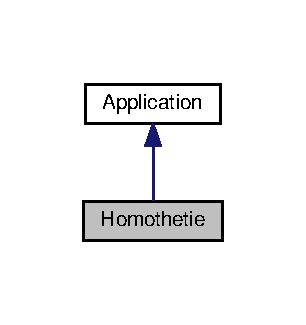
\includegraphics[width=147pt]{class_homothetie__inherit__graph}
\end{center}
\end{figure}


Graphe de collaboration de Homothetie\+:\nopagebreak
\begin{figure}[H]
\begin{center}
\leavevmode
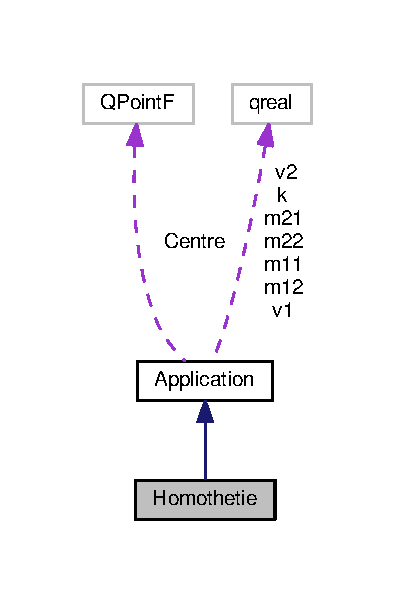
\includegraphics[width=190pt]{class_homothetie__coll__graph}
\end{center}
\end{figure}
\subsection*{Fonctions membres publiques}
\begin{DoxyCompactItemize}
\item 
\hypertarget{class_homothetie_a0c2ab7e4afc80bf76f10d6cecc2891fe}{}\hyperlink{class_homothetie_a0c2ab7e4afc80bf76f10d6cecc2891fe}{Homothetie} ()\label{class_homothetie_a0c2ab7e4afc80bf76f10d6cecc2891fe}

\begin{DoxyCompactList}\small\item\em \hyperlink{class_homothetie_a0c2ab7e4afc80bf76f10d6cecc2891fe}{Homothetie\+::\+Homothetie}. \end{DoxyCompactList}\item 
\hyperlink{class_homothetie_ab9e23a5bfa3141fde6951a4eec5cbe6e}{Homothetie} (qreal K)
\begin{DoxyCompactList}\small\item\em \hyperlink{class_homothetie_a0c2ab7e4afc80bf76f10d6cecc2891fe}{Homothetie\+::\+Homothetie}. \end{DoxyCompactList}\item 
\hyperlink{class_homothetie_a18b4271dabd8771540007efe8389827a}{Homothetie} (qreal K, Q\+Point\+F C)
\begin{DoxyCompactList}\small\item\em \hyperlink{class_homothetie_a0c2ab7e4afc80bf76f10d6cecc2891fe}{Homothetie\+::\+Homothetie}. \end{DoxyCompactList}\item 
void \hyperlink{class_homothetie_aa522cc6acd7c5822a67dde17e406da3c}{set\+Homothetie} (qreal K)
\begin{DoxyCompactList}\small\item\em \hyperlink{class_homothetie_aa522cc6acd7c5822a67dde17e406da3c}{Homothetie\+::set\+Homothetie}. \end{DoxyCompactList}\item 
void \hyperlink{class_homothetie_a759ed4ea817426a6f9aff78986b78bd1}{set\+Homothetie} (qreal K, Q\+Point\+F C)
\begin{DoxyCompactList}\small\item\em \hyperlink{class_homothetie_aa522cc6acd7c5822a67dde17e406da3c}{Homothetie\+::set\+Homothetie}. \end{DoxyCompactList}\end{DoxyCompactItemize}
\subsection*{Membres hérités additionnels}


\subsection{Documentation des constructeurs et destructeur}
\hypertarget{class_homothetie_ab9e23a5bfa3141fde6951a4eec5cbe6e}{}\index{Homothetie@{Homothetie}!Homothetie@{Homothetie}}
\index{Homothetie@{Homothetie}!Homothetie@{Homothetie}}
\subsubsection[{Homothetie}]{\setlength{\rightskip}{0pt plus 5cm}Homothetie\+::\+Homothetie (
\begin{DoxyParamCaption}
\item[{qreal}]{K}
\end{DoxyParamCaption}
)}\label{class_homothetie_ab9e23a5bfa3141fde6951a4eec5cbe6e}


\hyperlink{class_homothetie_a0c2ab7e4afc80bf76f10d6cecc2891fe}{Homothetie\+::\+Homothetie}. 


\begin{DoxyParams}{Paramètres}
{\em K} & \\
\hline
\end{DoxyParams}
\hypertarget{class_homothetie_a18b4271dabd8771540007efe8389827a}{}\index{Homothetie@{Homothetie}!Homothetie@{Homothetie}}
\index{Homothetie@{Homothetie}!Homothetie@{Homothetie}}
\subsubsection[{Homothetie}]{\setlength{\rightskip}{0pt plus 5cm}Homothetie\+::\+Homothetie (
\begin{DoxyParamCaption}
\item[{qreal}]{K, }
\item[{Q\+Point\+F}]{C}
\end{DoxyParamCaption}
)}\label{class_homothetie_a18b4271dabd8771540007efe8389827a}


\hyperlink{class_homothetie_a0c2ab7e4afc80bf76f10d6cecc2891fe}{Homothetie\+::\+Homothetie}. 


\begin{DoxyParams}{Paramètres}
{\em K} & \\
\hline
{\em C} & \\
\hline
\end{DoxyParams}


\subsection{Documentation des fonctions membres}
\hypertarget{class_homothetie_aa522cc6acd7c5822a67dde17e406da3c}{}\index{Homothetie@{Homothetie}!set\+Homothetie@{set\+Homothetie}}
\index{set\+Homothetie@{set\+Homothetie}!Homothetie@{Homothetie}}
\subsubsection[{set\+Homothetie}]{\setlength{\rightskip}{0pt plus 5cm}void Homothetie\+::set\+Homothetie (
\begin{DoxyParamCaption}
\item[{qreal}]{K}
\end{DoxyParamCaption}
)}\label{class_homothetie_aa522cc6acd7c5822a67dde17e406da3c}


\hyperlink{class_homothetie_aa522cc6acd7c5822a67dde17e406da3c}{Homothetie\+::set\+Homothetie}. 


\begin{DoxyParams}{Paramètres}
{\em K} & \\
\hline
\end{DoxyParams}
\hypertarget{class_homothetie_a759ed4ea817426a6f9aff78986b78bd1}{}\index{Homothetie@{Homothetie}!set\+Homothetie@{set\+Homothetie}}
\index{set\+Homothetie@{set\+Homothetie}!Homothetie@{Homothetie}}
\subsubsection[{set\+Homothetie}]{\setlength{\rightskip}{0pt plus 5cm}void Homothetie\+::set\+Homothetie (
\begin{DoxyParamCaption}
\item[{qreal}]{K, }
\item[{Q\+Point\+F}]{C}
\end{DoxyParamCaption}
)}\label{class_homothetie_a759ed4ea817426a6f9aff78986b78bd1}


\hyperlink{class_homothetie_aa522cc6acd7c5822a67dde17e406da3c}{Homothetie\+::set\+Homothetie}. 


\begin{DoxyParams}{Paramètres}
{\em K} & \\
\hline
{\em C} & \\
\hline
\end{DoxyParams}


La documentation de cette classe a été générée à partir des fichiers suivants \+:\begin{DoxyCompactItemize}
\item 
homothetie.\+h\item 
homothetie.\+cpp\end{DoxyCompactItemize}

\hypertarget{class_q_main_window}{}\section{Référence de la classe Q\+Main\+Window}
\label{class_q_main_window}\index{Q\+Main\+Window@{Q\+Main\+Window}}


Graphe d\textquotesingle{}héritage de Q\+Main\+Window\+:\nopagebreak
\begin{figure}[H]
\begin{center}
\leavevmode
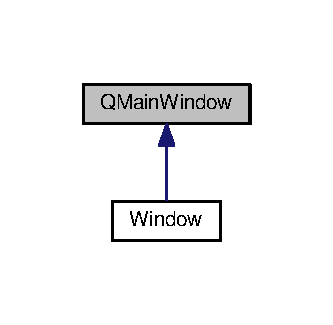
\includegraphics[width=160pt]{class_q_main_window__inherit__graph}
\end{center}
\end{figure}


La documentation de cette classe a été générée à partir du fichier suivant \+:\begin{DoxyCompactItemize}
\item 
\hyperlink{window_8h}{window.\+h}\end{DoxyCompactItemize}

\hypertarget{class_rotation}{}\section{Référence de la classe Rotation}
\label{class_rotation}\index{Rotation@{Rotation}}


{\ttfamily \#include \char`\"{}rotation.\+h\char`\"{}}



Graphe d\textquotesingle{}héritage de Rotation\+:\nopagebreak
\begin{figure}[H]
\begin{center}
\leavevmode
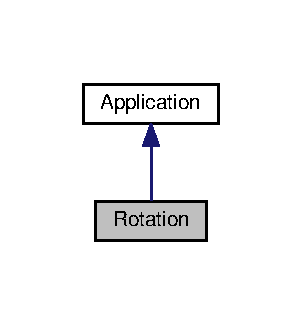
\includegraphics[width=145pt]{class_rotation__inherit__graph}
\end{center}
\end{figure}


Graphe de collaboration de Rotation\+:\nopagebreak
\begin{figure}[H]
\begin{center}
\leavevmode
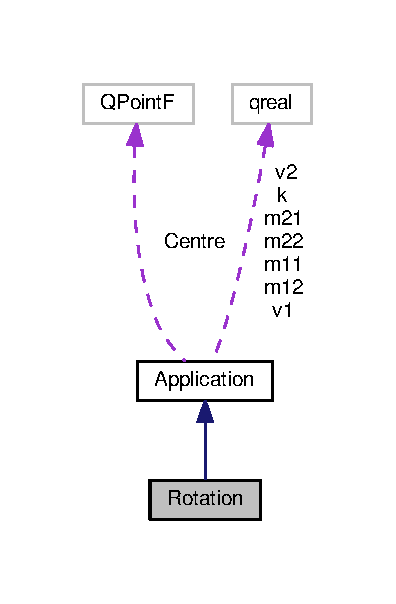
\includegraphics[width=190pt]{class_rotation__coll__graph}
\end{center}
\end{figure}
\subsection*{Fonctions membres publiques}
\begin{DoxyCompactItemize}
\item 
\hyperlink{class_rotation_a13ea1d345ca0a92c0f09b4de544ca460}{Rotation} ()
\begin{DoxyCompactList}\small\item\em \hyperlink{class_rotation_a13ea1d345ca0a92c0f09b4de544ca460}{Rotation\+::\+Rotation}. \end{DoxyCompactList}\item 
\hyperlink{class_rotation_a4939b65ee4d8cc83269eb668fc6aed40}{Rotation} (qreal theta)
\item 
\hyperlink{class_rotation_abfceda7f8e104a03351262fdf4c5356d}{Rotation} (qreal theta, Q\+Point\+F C)
\begin{DoxyCompactList}\small\item\em \hyperlink{class_rotation_a13ea1d345ca0a92c0f09b4de544ca460}{Rotation\+::\+Rotation}. \end{DoxyCompactList}\item 
void \hyperlink{class_rotation_ae4e808253ede637d1894f769778cd3cb}{set\+Rotation} (qreal theta)
\begin{DoxyCompactList}\small\item\em \hyperlink{class_rotation_ae4e808253ede637d1894f769778cd3cb}{Rotation\+::set\+Rotation}. \end{DoxyCompactList}\item 
void \hyperlink{class_rotation_aab9fbeda6f4a74f01d2418d232fbce44}{set\+Rotation} (qreal theta, Q\+Point\+F C)
\begin{DoxyCompactList}\small\item\em \hyperlink{class_rotation_ae4e808253ede637d1894f769778cd3cb}{Rotation\+::set\+Rotation}. \end{DoxyCompactList}\end{DoxyCompactItemize}
\subsection*{Membres hérités additionnels}


\subsection{Documentation des constructeurs et destructeur}
\hypertarget{class_rotation_a13ea1d345ca0a92c0f09b4de544ca460}{}\index{Rotation@{Rotation}!Rotation@{Rotation}}
\index{Rotation@{Rotation}!Rotation@{Rotation}}
\subsubsection[{Rotation}]{\setlength{\rightskip}{0pt plus 5cm}Rotation\+::\+Rotation (
\begin{DoxyParamCaption}
{}
\end{DoxyParamCaption}
)}\label{class_rotation_a13ea1d345ca0a92c0f09b4de544ca460}


\hyperlink{class_rotation_a13ea1d345ca0a92c0f09b4de544ca460}{Rotation\+::\+Rotation}. 

\hypertarget{class_rotation_a4939b65ee4d8cc83269eb668fc6aed40}{}\index{Rotation@{Rotation}!Rotation@{Rotation}}
\index{Rotation@{Rotation}!Rotation@{Rotation}}
\subsubsection[{Rotation}]{\setlength{\rightskip}{0pt plus 5cm}Rotation\+::\+Rotation (
\begin{DoxyParamCaption}
\item[{qreal}]{theta}
\end{DoxyParamCaption}
)}\label{class_rotation_a4939b65ee4d8cc83269eb668fc6aed40}
\hypertarget{class_rotation_abfceda7f8e104a03351262fdf4c5356d}{}\index{Rotation@{Rotation}!Rotation@{Rotation}}
\index{Rotation@{Rotation}!Rotation@{Rotation}}
\subsubsection[{Rotation}]{\setlength{\rightskip}{0pt plus 5cm}Rotation\+::\+Rotation (
\begin{DoxyParamCaption}
\item[{qreal}]{theta, }
\item[{Q\+Point\+F}]{C}
\end{DoxyParamCaption}
)}\label{class_rotation_abfceda7f8e104a03351262fdf4c5356d}


\hyperlink{class_rotation_a13ea1d345ca0a92c0f09b4de544ca460}{Rotation\+::\+Rotation}. 


\begin{DoxyParams}{Paramètres}
{\em theta} & \\
\hline
{\em C} & \\
\hline
\end{DoxyParams}


\subsection{Documentation des fonctions membres}
\hypertarget{class_rotation_ae4e808253ede637d1894f769778cd3cb}{}\index{Rotation@{Rotation}!set\+Rotation@{set\+Rotation}}
\index{set\+Rotation@{set\+Rotation}!Rotation@{Rotation}}
\subsubsection[{set\+Rotation}]{\setlength{\rightskip}{0pt plus 5cm}void Rotation\+::set\+Rotation (
\begin{DoxyParamCaption}
\item[{qreal}]{theta}
\end{DoxyParamCaption}
)}\label{class_rotation_ae4e808253ede637d1894f769778cd3cb}


\hyperlink{class_rotation_ae4e808253ede637d1894f769778cd3cb}{Rotation\+::set\+Rotation}. 


\begin{DoxyParams}{Paramètres}
{\em theta} & \\
\hline
\end{DoxyParams}
\hypertarget{class_rotation_aab9fbeda6f4a74f01d2418d232fbce44}{}\index{Rotation@{Rotation}!set\+Rotation@{set\+Rotation}}
\index{set\+Rotation@{set\+Rotation}!Rotation@{Rotation}}
\subsubsection[{set\+Rotation}]{\setlength{\rightskip}{0pt plus 5cm}void Rotation\+::set\+Rotation (
\begin{DoxyParamCaption}
\item[{qreal}]{theta, }
\item[{Q\+Point\+F}]{C}
\end{DoxyParamCaption}
)}\label{class_rotation_aab9fbeda6f4a74f01d2418d232fbce44}


\hyperlink{class_rotation_ae4e808253ede637d1894f769778cd3cb}{Rotation\+::set\+Rotation}. 


\begin{DoxyParams}{Paramètres}
{\em theta} & \\
\hline
{\em C} & \\
\hline
\end{DoxyParams}


La documentation de cette classe a été générée à partir des fichiers suivants \+:\begin{DoxyCompactItemize}
\item 
\hyperlink{rotation_8h}{rotation.\+h}\item 
\hyperlink{rotation_8cpp}{rotation.\+cpp}\end{DoxyCompactItemize}

\hypertarget{class_similitude_directe}{}\section{Référence de la classe Similitude\+Directe}
\label{class_similitude_directe}\index{Similitude\+Directe@{Similitude\+Directe}}


{\ttfamily \#include \char`\"{}similitudedirecte.\+h\char`\"{}}



Graphe d\textquotesingle{}héritage de Similitude\+Directe\+:\nopagebreak
\begin{figure}[H]
\begin{center}
\leavevmode
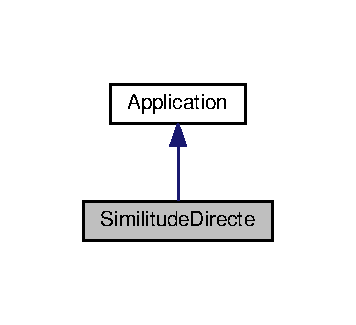
\includegraphics[width=171pt]{class_similitude_directe__inherit__graph}
\end{center}
\end{figure}


Graphe de collaboration de Similitude\+Directe\+:\nopagebreak
\begin{figure}[H]
\begin{center}
\leavevmode
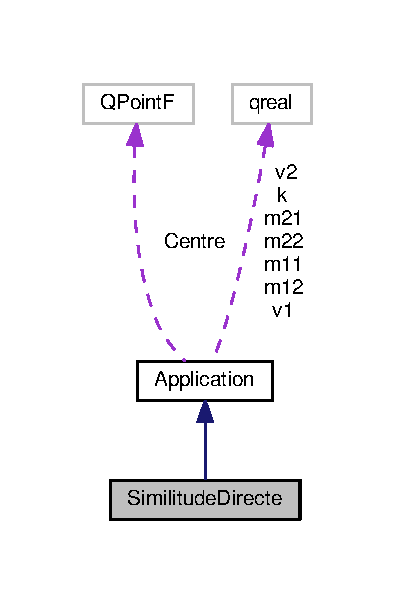
\includegraphics[width=190pt]{class_similitude_directe__coll__graph}
\end{center}
\end{figure}
\subsection*{Fonctions membres publiques}
\begin{DoxyCompactItemize}
\item 
\hyperlink{class_similitude_directe_a7ed5e906e0d9afa4eb5a50f26601b147}{Similitude\+Directe} ()
\begin{DoxyCompactList}\small\item\em \hyperlink{class_similitude_directe_a7ed5e906e0d9afa4eb5a50f26601b147}{Similitude\+Directe\+::\+Similitude\+Directe}. \end{DoxyCompactList}\item 
\hyperlink{class_similitude_directe_a64402a2d779eeedfd5f2ae86625daab5}{Similitude\+Directe} (qreal K, qreal theta, Q\+Point\+F C)
\begin{DoxyCompactList}\small\item\em \hyperlink{class_similitude_directe_a7ed5e906e0d9afa4eb5a50f26601b147}{Similitude\+Directe\+::\+Similitude\+Directe}. \end{DoxyCompactList}\item 
\hyperlink{class_similitude_directe_ad31aec6121a2508b176b32f816a7f5c3}{Similitude\+Directe} (qreal K, qreal theta, Q\+Point\+F C, Q\+Point\+F P)
\begin{DoxyCompactList}\small\item\em \hyperlink{class_similitude_directe_a7ed5e906e0d9afa4eb5a50f26601b147}{Similitude\+Directe\+::\+Similitude\+Directe}. \end{DoxyCompactList}\item 
void \hyperlink{class_similitude_directe_a2d8111830addbc8c5743d218b31ee627}{set\+Similitude\+Directe} (qreal K, qreal theta, Q\+Point\+F C)
\begin{DoxyCompactList}\small\item\em \hyperlink{class_similitude_directe_a2d8111830addbc8c5743d218b31ee627}{Similitude\+Directe\+::set\+Similitude\+Directe}. \end{DoxyCompactList}\item 
void \hyperlink{class_similitude_directe_a1ed9f92c74afc2fc51dfa149355dd3ef}{set\+Similitude\+Directe} (qreal K, qreal theta, Q\+Point\+F C, Q\+Point\+F P)
\begin{DoxyCompactList}\small\item\em \hyperlink{class_similitude_directe_a2d8111830addbc8c5743d218b31ee627}{Similitude\+Directe\+::set\+Similitude\+Directe}. \end{DoxyCompactList}\item 
void \hyperlink{class_similitude_directe_af64456a45860433f87d823a62fb2493d}{set\+Theta} (qreal theta)
\begin{DoxyCompactList}\small\item\em \hyperlink{class_similitude_directe_af64456a45860433f87d823a62fb2493d}{Similitude\+Directe\+::set\+Theta}. \end{DoxyCompactList}\end{DoxyCompactItemize}
\subsection*{Membres hérités additionnels}


\subsection{Documentation des constructeurs et destructeur}
\hypertarget{class_similitude_directe_a7ed5e906e0d9afa4eb5a50f26601b147}{}\index{Similitude\+Directe@{Similitude\+Directe}!Similitude\+Directe@{Similitude\+Directe}}
\index{Similitude\+Directe@{Similitude\+Directe}!Similitude\+Directe@{Similitude\+Directe}}
\subsubsection[{Similitude\+Directe}]{\setlength{\rightskip}{0pt plus 5cm}Similitude\+Directe\+::\+Similitude\+Directe (
\begin{DoxyParamCaption}
{}
\end{DoxyParamCaption}
)}\label{class_similitude_directe_a7ed5e906e0d9afa4eb5a50f26601b147}


\hyperlink{class_similitude_directe_a7ed5e906e0d9afa4eb5a50f26601b147}{Similitude\+Directe\+::\+Similitude\+Directe}. 

\hypertarget{class_similitude_directe_a64402a2d779eeedfd5f2ae86625daab5}{}\index{Similitude\+Directe@{Similitude\+Directe}!Similitude\+Directe@{Similitude\+Directe}}
\index{Similitude\+Directe@{Similitude\+Directe}!Similitude\+Directe@{Similitude\+Directe}}
\subsubsection[{Similitude\+Directe}]{\setlength{\rightskip}{0pt plus 5cm}Similitude\+Directe\+::\+Similitude\+Directe (
\begin{DoxyParamCaption}
\item[{qreal}]{K, }
\item[{qreal}]{theta, }
\item[{Q\+Point\+F}]{C}
\end{DoxyParamCaption}
)}\label{class_similitude_directe_a64402a2d779eeedfd5f2ae86625daab5}


\hyperlink{class_similitude_directe_a7ed5e906e0d9afa4eb5a50f26601b147}{Similitude\+Directe\+::\+Similitude\+Directe}. 


\begin{DoxyParams}{Paramètres}
{\em K} & \\
\hline
{\em theta} & \\
\hline
{\em C} & \\
\hline
\end{DoxyParams}
\hypertarget{class_similitude_directe_ad31aec6121a2508b176b32f816a7f5c3}{}\index{Similitude\+Directe@{Similitude\+Directe}!Similitude\+Directe@{Similitude\+Directe}}
\index{Similitude\+Directe@{Similitude\+Directe}!Similitude\+Directe@{Similitude\+Directe}}
\subsubsection[{Similitude\+Directe}]{\setlength{\rightskip}{0pt plus 5cm}Similitude\+Directe\+::\+Similitude\+Directe (
\begin{DoxyParamCaption}
\item[{qreal}]{K, }
\item[{qreal}]{theta, }
\item[{Q\+Point\+F}]{C, }
\item[{Q\+Point\+F}]{P}
\end{DoxyParamCaption}
)}\label{class_similitude_directe_ad31aec6121a2508b176b32f816a7f5c3}


\hyperlink{class_similitude_directe_a7ed5e906e0d9afa4eb5a50f26601b147}{Similitude\+Directe\+::\+Similitude\+Directe}. 


\begin{DoxyParams}{Paramètres}
{\em K} & \\
\hline
{\em theta} & \\
\hline
{\em C} & \\
\hline
{\em P} & \\
\hline
\end{DoxyParams}


\subsection{Documentation des fonctions membres}
\hypertarget{class_similitude_directe_a2d8111830addbc8c5743d218b31ee627}{}\index{Similitude\+Directe@{Similitude\+Directe}!set\+Similitude\+Directe@{set\+Similitude\+Directe}}
\index{set\+Similitude\+Directe@{set\+Similitude\+Directe}!Similitude\+Directe@{Similitude\+Directe}}
\subsubsection[{set\+Similitude\+Directe}]{\setlength{\rightskip}{0pt plus 5cm}void Similitude\+Directe\+::set\+Similitude\+Directe (
\begin{DoxyParamCaption}
\item[{qreal}]{K, }
\item[{qreal}]{theta, }
\item[{Q\+Point\+F}]{C}
\end{DoxyParamCaption}
)}\label{class_similitude_directe_a2d8111830addbc8c5743d218b31ee627}


\hyperlink{class_similitude_directe_a2d8111830addbc8c5743d218b31ee627}{Similitude\+Directe\+::set\+Similitude\+Directe}. 


\begin{DoxyParams}{Paramètres}
{\em K} & \\
\hline
{\em theta} & \\
\hline
{\em C} & \\
\hline
\end{DoxyParams}
\hypertarget{class_similitude_directe_a1ed9f92c74afc2fc51dfa149355dd3ef}{}\index{Similitude\+Directe@{Similitude\+Directe}!set\+Similitude\+Directe@{set\+Similitude\+Directe}}
\index{set\+Similitude\+Directe@{set\+Similitude\+Directe}!Similitude\+Directe@{Similitude\+Directe}}
\subsubsection[{set\+Similitude\+Directe}]{\setlength{\rightskip}{0pt plus 5cm}void Similitude\+Directe\+::set\+Similitude\+Directe (
\begin{DoxyParamCaption}
\item[{qreal}]{K, }
\item[{qreal}]{theta, }
\item[{Q\+Point\+F}]{C, }
\item[{Q\+Point\+F}]{P}
\end{DoxyParamCaption}
)}\label{class_similitude_directe_a1ed9f92c74afc2fc51dfa149355dd3ef}


\hyperlink{class_similitude_directe_a2d8111830addbc8c5743d218b31ee627}{Similitude\+Directe\+::set\+Similitude\+Directe}. 


\begin{DoxyParams}{Paramètres}
{\em K} & \\
\hline
{\em theta} & \\
\hline
{\em C} & \\
\hline
{\em P} & \\
\hline
\end{DoxyParams}
\hypertarget{class_similitude_directe_af64456a45860433f87d823a62fb2493d}{}\index{Similitude\+Directe@{Similitude\+Directe}!set\+Theta@{set\+Theta}}
\index{set\+Theta@{set\+Theta}!Similitude\+Directe@{Similitude\+Directe}}
\subsubsection[{set\+Theta}]{\setlength{\rightskip}{0pt plus 5cm}void Similitude\+Directe\+::set\+Theta (
\begin{DoxyParamCaption}
\item[{qreal}]{theta}
\end{DoxyParamCaption}
)}\label{class_similitude_directe_af64456a45860433f87d823a62fb2493d}


\hyperlink{class_similitude_directe_af64456a45860433f87d823a62fb2493d}{Similitude\+Directe\+::set\+Theta}. 


\begin{DoxyParams}{Paramètres}
{\em theta} & \\
\hline
\end{DoxyParams}


La documentation de cette classe a été générée à partir des fichiers suivants \+:\begin{DoxyCompactItemize}
\item 
\hyperlink{similitudedirecte_8h}{similitudedirecte.\+h}\item 
\hyperlink{similitudedirecte_8cpp}{similitudedirecte.\+cpp}\end{DoxyCompactItemize}

\hypertarget{class_similitude_indirecte}{}\section{Référence de la classe Similitude\+Indirecte}
\label{class_similitude_indirecte}\index{Similitude\+Indirecte@{Similitude\+Indirecte}}


{\ttfamily \#include \char`\"{}similitudeindirecte.\+h\char`\"{}}



Graphe d\textquotesingle{}héritage de Similitude\+Indirecte\+:\nopagebreak
\begin{figure}[H]
\begin{center}
\leavevmode
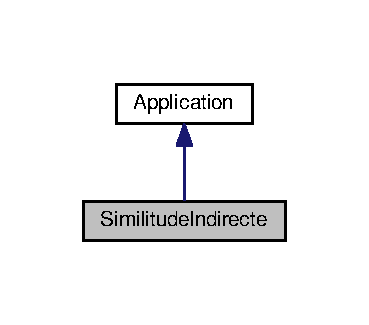
\includegraphics[width=177pt]{class_similitude_indirecte__inherit__graph}
\end{center}
\end{figure}


Graphe de collaboration de Similitude\+Indirecte\+:\nopagebreak
\begin{figure}[H]
\begin{center}
\leavevmode
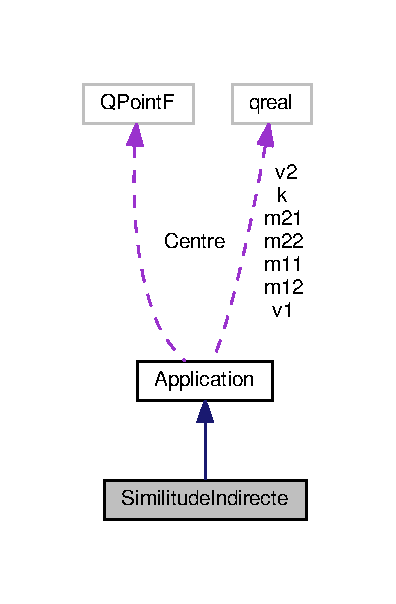
\includegraphics[width=190pt]{class_similitude_indirecte__coll__graph}
\end{center}
\end{figure}
\subsection*{Fonctions membres publiques}
\begin{DoxyCompactItemize}
\item 
\hyperlink{class_similitude_indirecte_a3f38af24b7ab4c26c96a6f67aa6b5ed4}{Similitude\+Indirecte} ()
\begin{DoxyCompactList}\small\item\em \hyperlink{class_similitude_indirecte_a3f38af24b7ab4c26c96a6f67aa6b5ed4}{Similitude\+Indirecte\+::\+Similitude\+Indirecte}. \end{DoxyCompactList}\item 
\hyperlink{class_similitude_indirecte_a163c2a1ce46d77570755e72c9e9b7ea6}{Similitude\+Indirecte} (qreal K, qreal theta, Q\+Point\+F P)
\begin{DoxyCompactList}\small\item\em \hyperlink{class_similitude_indirecte_a3f38af24b7ab4c26c96a6f67aa6b5ed4}{Similitude\+Indirecte\+::\+Similitude\+Indirecte}. \end{DoxyCompactList}\item 
\hyperlink{class_similitude_indirecte_a2d19403d78f488b0acaac269320176c4}{Similitude\+Indirecte} (qreal K, qreal theta, Q\+Point\+F P, Q\+Point\+F C)
\begin{DoxyCompactList}\small\item\em \hyperlink{class_similitude_indirecte_a3f38af24b7ab4c26c96a6f67aa6b5ed4}{Similitude\+Indirecte\+::\+Similitude\+Indirecte}. \end{DoxyCompactList}\item 
void \hyperlink{class_similitude_indirecte_aeacc6c5446e47385e70f385e6796f4ef}{set\+Similitude\+Indirecte} (qreal K, qreal theta, Q\+Point\+F P)
\begin{DoxyCompactList}\small\item\em \hyperlink{class_similitude_indirecte_aeacc6c5446e47385e70f385e6796f4ef}{Similitude\+Indirecte\+::set\+Similitude\+Indirecte}. \end{DoxyCompactList}\item 
void \hyperlink{class_similitude_indirecte_a0ca3f4cdc2eb804513fa46e1fbc8534f}{set\+Similitude\+Indirecte} (qreal K, qreal theta, Q\+Point\+F P, Q\+Point\+F C)
\begin{DoxyCompactList}\small\item\em \hyperlink{class_similitude_indirecte_aeacc6c5446e47385e70f385e6796f4ef}{Similitude\+Indirecte\+::set\+Similitude\+Indirecte}. \end{DoxyCompactList}\end{DoxyCompactItemize}
\subsection*{Membres hérités additionnels}


\subsection{Documentation des constructeurs et destructeur}
\hypertarget{class_similitude_indirecte_a3f38af24b7ab4c26c96a6f67aa6b5ed4}{}\index{Similitude\+Indirecte@{Similitude\+Indirecte}!Similitude\+Indirecte@{Similitude\+Indirecte}}
\index{Similitude\+Indirecte@{Similitude\+Indirecte}!Similitude\+Indirecte@{Similitude\+Indirecte}}
\subsubsection[{Similitude\+Indirecte}]{\setlength{\rightskip}{0pt plus 5cm}Similitude\+Indirecte\+::\+Similitude\+Indirecte (
\begin{DoxyParamCaption}
{}
\end{DoxyParamCaption}
)}\label{class_similitude_indirecte_a3f38af24b7ab4c26c96a6f67aa6b5ed4}


\hyperlink{class_similitude_indirecte_a3f38af24b7ab4c26c96a6f67aa6b5ed4}{Similitude\+Indirecte\+::\+Similitude\+Indirecte}. 

\hypertarget{class_similitude_indirecte_a163c2a1ce46d77570755e72c9e9b7ea6}{}\index{Similitude\+Indirecte@{Similitude\+Indirecte}!Similitude\+Indirecte@{Similitude\+Indirecte}}
\index{Similitude\+Indirecte@{Similitude\+Indirecte}!Similitude\+Indirecte@{Similitude\+Indirecte}}
\subsubsection[{Similitude\+Indirecte}]{\setlength{\rightskip}{0pt plus 5cm}Similitude\+Indirecte\+::\+Similitude\+Indirecte (
\begin{DoxyParamCaption}
\item[{qreal}]{K, }
\item[{qreal}]{theta, }
\item[{Q\+Point\+F}]{P}
\end{DoxyParamCaption}
)}\label{class_similitude_indirecte_a163c2a1ce46d77570755e72c9e9b7ea6}


\hyperlink{class_similitude_indirecte_a3f38af24b7ab4c26c96a6f67aa6b5ed4}{Similitude\+Indirecte\+::\+Similitude\+Indirecte}. 


\begin{DoxyParams}{Paramètres}
{\em K} & \\
\hline
{\em theta} & \\
\hline
{\em P} & \\
\hline
\end{DoxyParams}
\hypertarget{class_similitude_indirecte_a2d19403d78f488b0acaac269320176c4}{}\index{Similitude\+Indirecte@{Similitude\+Indirecte}!Similitude\+Indirecte@{Similitude\+Indirecte}}
\index{Similitude\+Indirecte@{Similitude\+Indirecte}!Similitude\+Indirecte@{Similitude\+Indirecte}}
\subsubsection[{Similitude\+Indirecte}]{\setlength{\rightskip}{0pt plus 5cm}Similitude\+Indirecte\+::\+Similitude\+Indirecte (
\begin{DoxyParamCaption}
\item[{qreal}]{K, }
\item[{qreal}]{theta, }
\item[{Q\+Point\+F}]{P, }
\item[{Q\+Point\+F}]{C}
\end{DoxyParamCaption}
)}\label{class_similitude_indirecte_a2d19403d78f488b0acaac269320176c4}


\hyperlink{class_similitude_indirecte_a3f38af24b7ab4c26c96a6f67aa6b5ed4}{Similitude\+Indirecte\+::\+Similitude\+Indirecte}. 


\begin{DoxyParams}{Paramètres}
{\em K} & \\
\hline
{\em theta} & \\
\hline
{\em P} & \\
\hline
{\em C} & \\
\hline
\end{DoxyParams}


\subsection{Documentation des fonctions membres}
\hypertarget{class_similitude_indirecte_aeacc6c5446e47385e70f385e6796f4ef}{}\index{Similitude\+Indirecte@{Similitude\+Indirecte}!set\+Similitude\+Indirecte@{set\+Similitude\+Indirecte}}
\index{set\+Similitude\+Indirecte@{set\+Similitude\+Indirecte}!Similitude\+Indirecte@{Similitude\+Indirecte}}
\subsubsection[{set\+Similitude\+Indirecte}]{\setlength{\rightskip}{0pt plus 5cm}void Similitude\+Indirecte\+::set\+Similitude\+Indirecte (
\begin{DoxyParamCaption}
\item[{qreal}]{K, }
\item[{qreal}]{theta, }
\item[{Q\+Point\+F}]{P}
\end{DoxyParamCaption}
)}\label{class_similitude_indirecte_aeacc6c5446e47385e70f385e6796f4ef}


\hyperlink{class_similitude_indirecte_aeacc6c5446e47385e70f385e6796f4ef}{Similitude\+Indirecte\+::set\+Similitude\+Indirecte}. 


\begin{DoxyParams}{Paramètres}
{\em K} & \\
\hline
{\em theta} & \\
\hline
{\em P} & \\
\hline
\end{DoxyParams}
\hypertarget{class_similitude_indirecte_a0ca3f4cdc2eb804513fa46e1fbc8534f}{}\index{Similitude\+Indirecte@{Similitude\+Indirecte}!set\+Similitude\+Indirecte@{set\+Similitude\+Indirecte}}
\index{set\+Similitude\+Indirecte@{set\+Similitude\+Indirecte}!Similitude\+Indirecte@{Similitude\+Indirecte}}
\subsubsection[{set\+Similitude\+Indirecte}]{\setlength{\rightskip}{0pt plus 5cm}void Similitude\+Indirecte\+::set\+Similitude\+Indirecte (
\begin{DoxyParamCaption}
\item[{qreal}]{K, }
\item[{qreal}]{theta, }
\item[{Q\+Point\+F}]{P, }
\item[{Q\+Point\+F}]{C}
\end{DoxyParamCaption}
)}\label{class_similitude_indirecte_a0ca3f4cdc2eb804513fa46e1fbc8534f}


\hyperlink{class_similitude_indirecte_aeacc6c5446e47385e70f385e6796f4ef}{Similitude\+Indirecte\+::set\+Similitude\+Indirecte}. 


\begin{DoxyParams}{Paramètres}
{\em K} & \\
\hline
{\em theta} & \\
\hline
{\em P} & \\
\hline
{\em C} & \\
\hline
\end{DoxyParams}


La documentation de cette classe a été générée à partir des fichiers suivants \+:\begin{DoxyCompactItemize}
\item 
\hyperlink{similitudeindirecte_8h}{similitudeindirecte.\+h}\item 
\hyperlink{similitudeindirecte_8cpp}{similitudeindirecte.\+cpp}\end{DoxyCompactItemize}

\hypertarget{class_window}{}\section{Référence de la classe Window}
\label{class_window}\index{Window@{Window}}


Graphe d\textquotesingle{}héritage de Window\+:\nopagebreak
\begin{figure}[H]
\begin{center}
\leavevmode
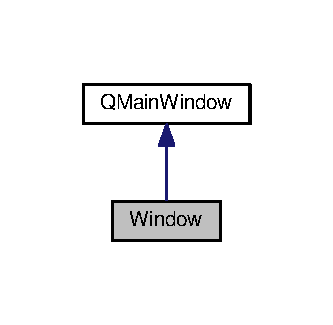
\includegraphics[width=160pt]{class_window__inherit__graph}
\end{center}
\end{figure}


Graphe de collaboration de Window\+:\nopagebreak
\begin{figure}[H]
\begin{center}
\leavevmode
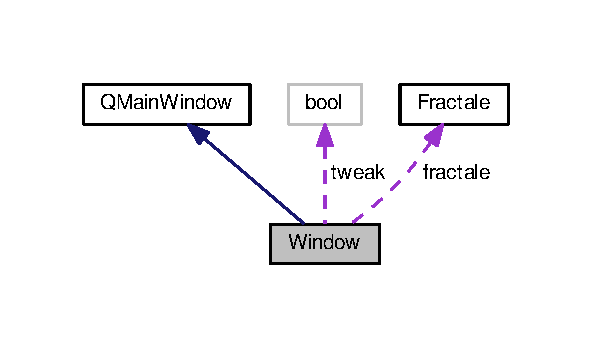
\includegraphics[width=284pt]{class_window__coll__graph}
\end{center}
\end{figure}
\subsection*{Connecteurs publics}
\begin{DoxyCompactItemize}
\item 
\hypertarget{class_window_a0c61ace2c0af9829fc1c66f96edf64be}{}void \hyperlink{class_window_a0c61ace2c0af9829fc1c66f96edf64be}{load} ()\label{class_window_a0c61ace2c0af9829fc1c66f96edf64be}

\begin{DoxyCompactList}\small\item\em \hyperlink{class_window_a0c61ace2c0af9829fc1c66f96edf64be}{Window\+::load}. \end{DoxyCompactList}\item 
\hypertarget{class_window_ab2babfe1d3ae399e069000309cc3a7ae}{}void \hyperlink{class_window_ab2babfe1d3ae399e069000309cc3a7ae}{refresh\+View} ()\label{class_window_ab2babfe1d3ae399e069000309cc3a7ae}

\begin{DoxyCompactList}\small\item\em \hyperlink{class_window_ab2babfe1d3ae399e069000309cc3a7ae}{Window\+::refresh\+View}. \end{DoxyCompactList}\end{DoxyCompactItemize}
\subsection*{Fonctions membres publiques}
\begin{DoxyCompactItemize}
\item 
\hypertarget{class_window_a74e6087da23d3c24e9fac0245e5ec92c}{}\hyperlink{class_window_a74e6087da23d3c24e9fac0245e5ec92c}{Window} ()\label{class_window_a74e6087da23d3c24e9fac0245e5ec92c}

\begin{DoxyCompactList}\small\item\em \hyperlink{class_window_a74e6087da23d3c24e9fac0245e5ec92c}{Window\+::\+Window}. \end{DoxyCompactList}\end{DoxyCompactItemize}
\subsection*{Attributs publics}
\begin{DoxyCompactItemize}
\item 
\hypertarget{class_window_a52e7d4e63f98e761696b4e5e0296c053}{}bool {\bfseries tweak}\label{class_window_a52e7d4e63f98e761696b4e5e0296c053}

\item 
\hypertarget{class_window_a022688408d51ba601784ebfef3f8da10}{}\hyperlink{class_fractale}{Fractale} $\ast$ {\bfseries fractale}\label{class_window_a022688408d51ba601784ebfef3f8da10}

\end{DoxyCompactItemize}
\subsection*{Fonctions membres protégées}
\begin{DoxyCompactItemize}
\item 
virtual bool \hyperlink{class_window_a7c7748b81d769f66a2131c2f66541da9}{event\+Filter} (Q\+Object $\ast$obj, Q\+Event $\ast$event)
\begin{DoxyCompactList}\small\item\em \hyperlink{class_window_a7c7748b81d769f66a2131c2f66541da9}{Window\+::event\+Filter}. \end{DoxyCompactList}\end{DoxyCompactItemize}


\subsection{Documentation des fonctions membres}
\hypertarget{class_window_a7c7748b81d769f66a2131c2f66541da9}{}\index{Window@{Window}!event\+Filter@{event\+Filter}}
\index{event\+Filter@{event\+Filter}!Window@{Window}}
\subsubsection[{event\+Filter}]{\setlength{\rightskip}{0pt plus 5cm}bool Window\+::event\+Filter (
\begin{DoxyParamCaption}
\item[{Q\+Object $\ast$}]{obj, }
\item[{Q\+Event $\ast$}]{event}
\end{DoxyParamCaption}
)\hspace{0.3cm}{\ttfamily [protected]}, {\ttfamily [virtual]}}\label{class_window_a7c7748b81d769f66a2131c2f66541da9}


\hyperlink{class_window_a7c7748b81d769f66a2131c2f66541da9}{Window\+::event\+Filter}. 


\begin{DoxyParams}{Paramètres}
{\em obj} & \\
\hline
{\em event} & \\
\hline
\end{DoxyParams}
\begin{DoxyReturn}{Renvoie}

\end{DoxyReturn}


La documentation de cette classe a été générée à partir des fichiers suivants \+:\begin{DoxyCompactItemize}
\item 
window.\+h\item 
window.\+cpp\end{DoxyCompactItemize}

%--- End generated contents ---

% Index
\backmatter
\newpage
\phantomsection
\clearemptydoublepage
\addcontentsline{toc}{chapter}{Index}
\printindex

\end{document}
